\section{Introduction}
In 1828, an English mathematician named George Green published ``An Essay on the Application of Mathematical Analysis to the Theories of Electricity and Magnetism" with a theorem that is now used extensively to solve differential equations in electromagnetics, quantum mechanics, and applied mathematics \cite{green_phys_today}. Today Green's functions are a useful tool in solving inhomogeneous differential equations and can be thought of as an impulse response. There are many references for Green's functions from the mathematical perspective \cite{bender_orszag}, \cite{arfken_weber}, \cite{gbur_math}, \cite{guenther_partial_de}, \cite{duffy_green}, and for their application to electromagnetics \cite{jackson_classical_em}, \cite{zangwill_modern_em}, \cite{balanis_advanced}, \cite{goodman_fourier}, \cite{smith_radiation}, \cite{schwinger_em}. Unfortunately, these references are by necessity specialized, only highlighting one aspect and skipping over significant steps. In addition, they often have conflicting conventions for normalization and propagation direction. 

The purpose of this document is to fill this gap; presenting the theory behind Green's functions and demonstrating in a consistent manner how they can be used in electromagnetic propagation and diffraction problems. A particular emphasis is given to applications concerning the propagation of Radio Frequency (RF) waves in maritime environments and diffraction from the sea surface. The discussion will be restricted to scalar analysis and will not address dyadic forms, series expansions, or stochastic integrals.

\subsection{Time Dependence Sign Convention} \label{gf_sec:time_dependence}
Before getting started, we need to define the sign convention used for time dependence. We  assume harmonic propagating waves that follow the typical engineering literature with time dependence going as $e^{j\omega t}$. This choice of time dependence defines the spatial dependence and the forward and reverse Fourier transforms in both the temporal and spatial domains.

For a system to be causal, it may only depend on past or present inputs and not on future inputs. Any physically realizable system, such as an electromagnetic wave, must be causal as something that has not yet happened cannot have an impact on the current output. We can relate the causality condition to the phase with the restriction that the phase can be delayed but not advanced. This tells us that for propagating waves, we need to look for solutions in the form of $g\left(\pm\left[\omega t - k_or\right]\right)$, as solutions in the form of $g\left(\pm\left[\omega t + k_or\right]\right)$ advance the phase and are not physically realizable. 

With this restriction, an arbitrary vector wave, $\mathbf{C}$ must take the form:

\begin{equation}
\mathbf{C}\left(\mathbf{r},t\right) = \mathbf{C}e^{j\left(\omega t - \mathbf{k}_o \cdot \mathbf{r} \right)}
\label{gf_eq:18b}
\end{equation}
\renewcommand{\baselinestretch}{2} \small\normalsize

\subsection {Fourier Transforms in Time and Space} \label{gf_sec:fourier_transform}
As a mathematical construct, the signs on the forward and reverse Fourier transforms are irrelevant as long as we are consistent when moving into and out of the frequency domain. In physics however, we must remain consistent with the conventions we have established. The easiest way to do so is to interpret the transform from a frequency domain to either the temporal or spatial domain as a superposition of the signal of interest with forward propagating waves over all frequencies. The sign convention for the inverse Fourier transform then comes directly from our definition of a forward propagating wave from the previous section.  

Table \ref{gf_tab:0a} presents the forward Fourier transforms, $\hat{g} = \mathcal{F}\{g\}$, and the inverse Fourier transforms, $g = \mathcal{F}^{-1}\{\hat{g}\}$, in both time and space for an arbitrary function, $g$, and its Fourier transform, $\hat{g}$.

\begin{table}[ht]
  \centering
      %\renewcommand{\baselinestretch}{1} \small\normalsize
  \begin{quote}
    \caption[Fourier Transforms in Time and Space]{Fourier Transforms in Time and Space\label{gf_tab:0a}}
  \end{quote}
  \begin{tabular} {|c | c | c|}
    \hline
  \bf{Domain} & \bf{Forward Transform} & \bf{Inverse Transform}\\ \hline
  Time & $\displaystyle \hat{g}(\omega) = \int_{-\infty}^{\infty} g(t)e^{-j\omega t}dt$ & $\displaystyle  g(t) = \frac{1}{2\pi}\int_{-\infty}^\infty \hat{g}(\omega)e^{j\omega t}d\omega$\\[5pt] \hline
 Space & $\displaystyle \hat{g}(k) = \int_{-\infty}^{\infty} g(x)e^{jk x}dx$ & $\displaystyle  g(x) = \frac{1}{2\pi}\int_{-\infty}^\infty \hat{g}(k)e^{-jk x}dk$\\[5pt] \hline
\end{tabular}

\end{table}
\renewcommand{\baselinestretch}{2} \small\normalsize

\subsection{Geometric Spreading}
When using mathematical models of electromagnetic wave propagation, the amount of geometric spreading is dependent on the dimensionality and approximations used. A plane wave is easy to work with but is not physically realizable and shows no spreading or amplitude reduction as it propagates. A paraxial wave allows us to represent beam like waves and will have spreading proportional to $1/\sqrt{L_x}$, where $L_x$ is the length along the propagation direction (for propagation over the earth, this can be interpreted as the ground distance between points). A cylindrical wave will have spreading proportional to $1/\sqrt{\rho}$ and a spherical wave will have spreading proportional to $1/r$, where $\rho$ and $r$ are the respective path lengths in the corresponding coordinate system. These differences do not necessarily mean an answer is wrong, but indicate we need to understand the limitations of any model we choose.

\subsection{Common Pitfalls}
There are several potential issues that need to be considered when analyzing any propagation problem. The following list is certainly not exhaustive, but captures some tripping points that may be encountered.

\begin{enumerate}
\item Consistency with Fourier transform definitions. As previously discussed, the time and space versions of Fourier transforms will have opposing signs due to causality. When using numerical Fast Fourier Transform (FFT) implementations, we need to ensure they match the conventions used as described in Table \ref{gf_tab:0a}.
\item Polarization effects are not captured in scalar propagation. Because we are restricting the analysis to scalar propagation, there is no sense of polarization. This means that once set, the polarization will be constant for all time. Amplitude changes for the current polarization are accounted for through the reflection coefficients and boundary conditions as those implicitly have polarization dependence.
\item No backscattering with paraxial approximation. The paraxial assumption greatly simplifies analysis and is extremely useful for describing beam like waves, Fresnel and Fraunhofer diffraction, and the parabolic wave equation (PWE). However, this assumption effectively factors out backward propagating waves and only provides solutions for forward propagating waves. This means that with the paraxial assumption, we do not get any kind of backward scattering in the solution and will need to supplement the results where backscattering is important (e.g. clutter). 
\end{enumerate}

\section {Green's Identities and Method}
The two identities named for George Green and the method of Green’s functions will be derived here.

\subsection{Identities}
To derive Green’s identities, we start with the divergence theorem:

\begin{equation}
\oint\limits_{S} \mathbf{C} \cdot \hat{n} dS = \int\limits_{V}d^3r'\nabla \cdot \mathbf{C}
\label{gf_eq:1}
\end{equation}
\renewcommand{\baselinestretch}{2} \small\normalsize

By replacing the vector $\mathbf{C}$ with a function of two arbitrary scalar variables, $\mathbf{C}=\varphi\nabla\psi$, we get:

\begin{equation}
\oint\limits_{S} \varphi\nabla\psi \cdot \hat{n} dS = \int\limits_{V}d^3r'\nabla \cdot \varphi\nabla\psi
\label{gf_eq:2}
\end{equation}
\renewcommand{\baselinestretch}{2} \small\normalsize

Using the identity $\nabla\psi\cdot \hat{n} = \partial \psi/\partial n$ and expanding the dot product in the volume integral yields Green's first identity:

\begin{equation}
\boxed{\oint\limits_{S} \varphi\frac{\partial \psi}{\partial n} dS = \int\limits_{V}d^3r' \left[ \nabla\varphi \cdot \nabla\psi +\varphi \nabla^2 \psi\right]}
\label{gf_eq:3}
\end{equation}
\renewcommand{\baselinestretch}{2} \small\normalsize

If we flip the order of the scalar variables and instead let $\mathbf{C}=\psi\nabla\varphi$, Green's first identity is expressed as:

\begin{equation}
\oint\limits_{S} \psi\frac{\partial \varphi}{\partial n} dS = \int\limits_{V}d^3r' \left[ \nabla\psi \cdot \nabla\varphi +\psi \nabla^2 \varphi\right]
\label{gf_eq:4}
\end{equation}
\renewcommand{\baselinestretch}{2} \small\normalsize

\noindent Subtracting Equation \ref{gf_eq:4} from Equation \ref{gf_eq:3} yields Green's second identity:

\begin{equation}
\boxed{\oint\limits_{S} \left[ \varphi\frac{\partial \psi}{\partial n} - \psi\frac{\partial \varphi}{\partial n} \right]dS = \int\limits_{V}d^3r' \left[ \varphi\nabla^2\psi- \psi \nabla^2 \varphi\right]}
\label{gf_eq:5}
\end{equation}

\subsection {Method of Green's Functions} \label{gf_sec:method}
Since we are interested in propagation problems, we would like to apply the method of Green's functions to the scalar wave equation  to solve for the scalar field, $\varphi$, as a function of space and time with an arbitrary driving function, $f$, that is also a function of space and time:

\begin{equation}
\nabla^2\varphi\left(\mathbf{r},t\right) - \frac{n_r^2}{c^2}\frac{\partial^2 \varphi\left(\mathbf{r},t\right)}{\partial t^2} = f\left(\mathbf{r},t\right)
\label{gf_eq:6}
\end{equation}
\renewcommand{\baselinestretch}{2} \small\normalsize

\noindent Assuming the index of refraction, $n_r$, is constant in time, we can utilize the Fourier transform to remove the time dependence:

\begin{equation}
\nabla^2\varphi\left(\mathbf{r},\omega\right) + \frac{\omega^2n_r^2}{c^2}\varphi\left(\mathbf{r},\omega\right) = f\left(\mathbf{r},\omega\right)
\label{gf_eq:7}
\end{equation}
\renewcommand{\baselinestretch}{2} \small\normalsize

Equation \ref{gf_eq:7} is the Helmholtz equation and it represents the wave equation with only spatial derivatives. If we use the wave number, $k_o = \omega n_r/c$, and suppress the variable dependence for clarity, Equation \ref{gf_eq:7} can be rewritten as:

\begin{equation}
\nabla^2\varphi + k_o^2\varphi = f
\label{gf_eq:8}
\end{equation}
\renewcommand{\baselinestretch}{2} \small\normalsize

The Green's function for this problem can be found by replacing the driving function, $f$, with a delta function:

\begin{equation}
\nabla^2G+ k_o^2G = -\delta\left(\mathbf{r}-\mathbf{r}' \right)
\label{gf_eq:9}
\end{equation}
\renewcommand{\baselinestretch}{2} \small\normalsize

Equation \ref{gf_eq:9} shows that the Green's function is the solution to the differential equation for a spatial impulse and therefore represents the impulse response of the system. In electromagnetics, the driving force often has a negative sign as seen from the Poisson equation, $\nabla^2\varphi = -\rho/\epsilon_o$, so we typically chose a matching negative sign for the delta function. With this convention, we need to make sure the driving force has a negative sign when utilizing a Green's function later.

The general method to find Green's functions is to solve the homogeneous differential equation away from the delta function source and then integrate over a small region that includes the delta function for normalization. Some authors, such as \cite{jackson_classical_em} and \cite{schwinger_em}, include a $4\pi$ scale factor with the delta function to absorb this normalization term into the differential equation rather than the Green's function.

Equations \ref{gf_eq:8} and \ref{gf_eq:9} can be rearranged to solve for the Laplacian, so that $\nabla^2\varphi = f - k_o^2\varphi$ and $\nabla^2G = -\delta\left(\mathbf{r}-\mathbf{r}' \right) - k_o^2G$. We can substitute these values into Green's second identity (Equation \ref{gf_eq:5}), with $\psi=G$:

\begin{equation}
\begin{gathered}
\oint\limits_{S} \left[ \varphi\frac{\partial G}{\partial n} - G\frac{\partial \varphi}{\partial n} \right]dS = \int\limits_{V}d^3r' \left[ \varphi\nabla^2G- G \nabla^2 \varphi\right] \\
\oint\limits_{S} \left[ \varphi\frac{\partial G}{\partial n} - G\frac{\partial \varphi}{\partial n} \right]dS = \int\limits_{V}d^3r' \left[ \varphi \left(-\delta\left(\mathbf{r}-\mathbf{r}' \right) - k_o^2n_r^2G\right)- G \left(f - k_o^2\varphi \right)\right] \\
\end{gathered}
\label{gf_eq:10}
\end{equation}
\renewcommand{\baselinestretch}{2} \small\normalsize

Moving the volume integral over the delta function to the left hand side yields:

\begin{equation}
\begin{gathered}
\int\limits_{V}d^3r'\varphi\delta\left(\mathbf{r}-\mathbf{r}' \right) = \oint\limits_{S}\left[G\frac{\partial \varphi}{\partial n} - \varphi\frac{\partial G}{\partial n} \right]dS +\int\limits_{V}d^3r'\left[ Gk_o^2\varphi - \varphi k_o^2G - Gf \right] \\
\int\limits_{V}d^3r'\varphi\delta\left(\mathbf{r}-\mathbf{r}' \right) = \oint\limits_{S}\left[G\frac{\partial \varphi}{\partial n} - \varphi\frac{\partial G}{\partial n} \right]dS -\int\limits_{V}d^3r' Gf
\end{gathered}
\label{gf_eq:10a}
\end{equation}
\renewcommand{\baselinestretch}{2} \small\normalsize

As long as $\mathbf{r}'$ is in the volume $V$, we can use the sifting property of the delta function to provide an explicit representation for $\varphi$:

\begin{equation}
\boxed{\varphi = \oint\limits_{S}dS\left[G\frac{\partial \varphi}{\partial n} - \varphi\frac{\partial G}{\partial n} \right] -\int\limits_{V}d^3r' Gf}
\label{gf_eq:11}
\end{equation}
\renewcommand{\baselinestretch}{2} \small\normalsize

Equation \ref{gf_eq:11} defines the general solution for an inhomogeneous differential equation and the only assumption made here is that the forcing function will have a negative sign. The homogeneous solution is given by the surface integral and the response to a forcing function is given by the volume integral. When there are no boundary conditions (as in free space propagation), the normal derivatives are all zero so the surface integral vanishes and we are left with only the term due to the forcing function.

\begin{equation}
\varphi = -\int\limits_{V}d^3r' Gf
\label{gf_eq:11aa}
\end{equation}
\renewcommand{\baselinestretch}{2} \small\normalsize

In the simplest case, $f$ is a point source located at $r_o$ and can be represented by a delta function with a scalar amplitude, $ f = -\alpha\delta(r'-r_o)$, so that

\begin{equation}
\varphi = \alpha G(r,r_o)
\label{gf_eq:11ab}
\end{equation}
\renewcommand{\baselinestretch}{2} \small\normalsize

\section {Boundary Conditions}
There are two traditional types of boundary conditions: Dirichlet, where $\varphi$ is specified on the boundary, or Neuman, where the normal derivative of $\varphi$ is specified on the boundary. There is also a third type of boundary condition, known as the Robin condition, that is a weighted combination of Dirichlet and Neuman boundary conditions.

\subsection {Dirichlet Boundary Conditions}
For Dirichlet boundary conditions, the solution is specified on the surface, $\varphi\left(\mathbf{r}\right) |_{S} = \varphi\left(\mathbf{r}_S \right) = a\left(\mathbf{r}_s\right)$. To simplify Equation \ref{gf_eq:11}, we can apply a Dirichlet boundary condition on the Green’s function to remove the $\partial \varphi /\partial n$ dependence and leave only the known term in the surface integral.

\begin{equation}
G\left(\mathbf{r},\mathbf{r}' \right)\bigg|_{S}=0
\label{gf_eq:12}
\end{equation}
\renewcommand{\baselinestretch}{2} \small\normalsize

Substituting Equation \ref{gf_eq:12} into Equation \ref{gf_eq:11} results in the following equation for $\varphi$ in the presence of Dirichlet boundary conditions.

\begin{equation}
\boxed{\varphi = -\oint\limits_{S}dS \varphi\frac{\partial G}{\partial n} -\int\limits_{V}d^3r' Gf}
\label{gf_eq:13}
\end{equation}
\renewcommand{\baselinestretch}{2} \small\normalsize

Green's functions with Dirichlet boundary conditions are sometimes called Green's functions of the first kind and occur naturally in electrostatics and propagation over a Perfect Electrical Conductor (PEC). 

\subsection {Neuman Boundary Conditions}
For Neuman boundary conditions, the normal derivative of the field is specified on the surface, $\partial\varphi\left(\mathbf{r}\right)/\partial n|_{S} = b\left(\mathbf{r}_s\right)$. As described in \cite{jackson_classical_em}, \cite{zangwill_modern_em}, and \cite{balanis_advanced}, we cannot simply set the normal derivative of $G$ to $0$. This can be demonstrated by integrating Equation \ref{gf_eq:9} over a volume and then applying the divergence theorem:

\begin{equation}
\begin{gathered}
\int\limits_{V}d^3r' \nabla^2 G = \int\limits_{V}d^3r'\left[-\delta\left(\mathbf{r}-\mathbf{r}' \right) -k_o^2G \right] \\
\int\limits_{V}d^3r' \nabla \cdot \nabla G = -\int\limits_{V}d^3r'\delta\left(\mathbf{r}-\mathbf{r}' \right) -\int\limits_{V}d^3r'k_o^2G \\
\oint\limits_{S}\nabla G \cdot \hat{n} dS  = -1 - \int\limits_{V}d^3r'k_o^2G\\
\oint\limits_{S}\frac{\partial G}{\partial n} dS = -1 - \int\limits_{V}d^3r' k_o^2G
\end{gathered}
\label{gf_eq:14}
\end{equation}
\renewcommand{\baselinestretch}{2} \small\normalsize

The continuity and reciprocity properties that will be discussed in the next section ensure that the volume integral over $G$ vanishes, so we are left with the following general condition:

\begin{equation}
\oint\limits_{S}\frac{\partial G}{\partial n} dS = -1
\label{gf_eq:15}
\end{equation}
\renewcommand{\baselinestretch}{2} \small\normalsize

Equation \ref{gf_eq:15} indicates that there is a discontinuity in the normal derivative of the Green's function. Letting $S$ be the total surface area gives us the following condition on the normal derivative of the Green's function:

\begin{equation}
\frac{\partial G}{\partial n} = -\frac{1}{S}
\label{gf_eq:16}
\end{equation}
\renewcommand{\baselinestretch}{2} \small\normalsize

Equation \ref{gf_eq:16} demonstrates the jump condition for the normal derivative of the Green's function and we should note that when the surface is taken out to infinity that $\partial G/\partial n = 0$. Substituting Equation \ref{gf_eq:16} into Equation \ref{gf_eq:11} results in the following equation for $\varphi$ in the presence of Neuman boundary conditions.

\begin{equation}
\boxed{\varphi = \oint\limits_{S}dS\left[G\frac{\partial \varphi}{\partial n} + \frac{\varphi}{S} \right] -\int\limits_{V}d^3r' Gf}
\label{gf_eq:17}
\end{equation}
\renewcommand{\baselinestretch}{2} \small\normalsize

We can rewrite Equation \ref{gf_eq:17} as in \cite{jackson_classical_em}, using the average value of the solution over the surface, $\left< \varphi\right> = S^{-1}\oint\limits_{S}\varphi dS$:

\begin{equation}
\boxed{\varphi = \left<\varphi \right> + \oint\limits_{S}G\frac{\partial \varphi}{\partial n}dS  -\int\limits_{V}d^3r' Gf}
\label{gf_eq:18}
\end{equation}
\renewcommand{\baselinestretch}{2} \small\normalsize

Green's functions with Neuman boundary conditions are sometimes called Green's functions of the second kind and occur naturally in waveguides. 

\subsection {Robin Boundary Conditions}
For Robin boundary conditions, a weighted linear combination of the solution and its derivative are specified on the surface, $\partial\varphi\left(\mathbf{r}\right)/\partial n|_{S} +\alpha\varphi\left(\mathbf{r}\right) |_{S}= c\left(\mathbf{r}_s\right)$. 

We can generally set $c=0$ so that the Robin boundary condition relates the Green's function on the surface to its normal derivative on the surface.

\begin{equation}
\frac{\partial G\left(\mathbf{r}\right)}{\partial n}\bigg|_{S} = -\alpha G
\label{gf_eq:18aa}
\end{equation}
\renewcommand{\baselinestretch}{2} \small\normalsize

Substituting Equation \ref{gf_eq:18aa} into Equation \ref{gf_eq:11} results in the following equation for $\varphi$ in the presence of Robin boundary conditions.

\begin{equation}
\boxed{\varphi = \oint\limits_{S}dS\left[\frac{\partial \varphi}{\partial n} + \alpha\varphi \right]G -\int\limits_{V}d^3r' Gf}
\label{gf_eq:18aabb}
\end{equation}
\renewcommand{\baselinestretch}{2} \small\normalsize

Robin boundary conditions are commonly found in propagation problems with mixed polarization and cavities with apertures. They generally do not have simple solutions are usually solved numerically.

\section {Properties of Green's Functions} \label{gf_sec:properties}
We have already discussed the fact that a Green's function represents the spatial impulse response of a differential equation. This section introduces some other properties of Green's functions, including causality, reciprocity, continuity, and general forms.

\subsection {Causality} \label{gf_sec:causality}
Green's functions represent physical systems and therefore must be causal. With the time dependence as specified in Section \ref{gf_sec:time_dependence}, they must have the following form:

\begin{equation}
G\left(r,t\right) \sim g\left(\omega t - k_or\right)
\label{gf_eq:18a}
\end{equation}
\renewcommand{\baselinestretch}{2} \small\normalsize

\subsection {Reciprocity} \label{gf_sec:reciprocity}
Green's functions must be symmetric with respect to $\mathbf{r}$ (the vector to the observer) and $\mathbf{r}'$ (the vector to the source), so that:

\begin{equation}
G\left(\mathbf{r},\mathbf{r}' \right) = G\left(\mathbf{r}',\mathbf{r} \right)
\label{gf_eq:18c}
\end{equation}
\renewcommand{\baselinestretch}{2} \small\normalsize

This property is known as reciprocity and it tells us that the impulse reponse for a propagating wave is the same in both directions. Reciprocity is commonly used in antenna radiation analysis as it allows us to analyze an antenna considering it as either a transmitter or a receiver.

\subsection {Continuity} \label{gf_sec:continuity}
A necessary condition for reciprocity is that Green's functions must be continuous in all space. However, they are singular so the derivative will have a discontinuity at $\mathbf{r} = \mathbf{r}'$.

\subsection {General Forms}
Because a Green's function is the spatial impulse response of the system, we can expect it to be used in a convolution integral. With that in mind, Green's functions usually take the form:
\begin{equation}
G\left(\mathbf{r},\mathbf{r}' \right) = g\left( \mathbf{r} - \mathbf{r}'\right)
\label{gf_eq:18d}
\end{equation}
\renewcommand{\baselinestretch}{2} \small\normalsize

Using the results of the previously described properties, the most general representation of a Green's function is as follows:

\begin{equation}
G\left(\mathbf{r},\mathbf{r}',t ,t'\right) = g\left(\omega |t-t'| - k_o| \mathbf{r} - \mathbf{r}' | \right)
\label{gf_eq:19b}
\end{equation}
\renewcommand{\baselinestretch}{2} \small\normalsize

\section {Free Space Green's Functions}
This section derives the free space Green's functions for the Helmholtz equation (Equation \ref{gf_eq:9}) in both 3-dimensions and 2-dimensions. In the 2-dimensional case, we will also derive the Green's function for the paraxial wave equation. In free space, there are no boundaries, so we can let $r\rightarrow \infty$ and use Dirichlet boundary conditions at $\infty$. Without loss of generality, we can place the delta function at the origin, so that $\delta\left(\mathbf{r}-\mathbf{r}' \right) \rightarrow \delta \left(\mathbf{r} \right)$. To find the Green's function, we need to solve the homogeneous equation away from the delta function and then integrate over a small region around the origin for normalization. The homogenous equation to solve is:

\begin{equation}
\nabla^2G+ k_o^2G = 0
\label{gf_eq:19}
\end{equation}
\renewcommand{\baselinestretch}{2} \small\normalsize

Because the delta function is rotationally symmetric, the Green's function must also be rotationally symmetric.

\subsection {3-Dimensions}\label{gf_sec:3d}
This section derives the free space Green's function for the Helmholtz equation in 3-dimensional space. Because we used the Fourier transform to remove the time dependence from the wave equation (Equation 
\ref{gf_eq:6}), we will first work in the frequency domain and then transform the result back to the time domain.

\subsubsection {Deriviation in the Frequency Domain}
In 3-dimensions,  rotational symmetry means that  $\partial G/\partial\theta = \partial G/\partial\phi=0$. Therefore we can expand the Laplacian of Equation \ref{gf_eq:19} in spherical coordinates and neglect the $\theta$ and $\phi$ components:

\begin{equation}
\frac{1}{r^2}\frac{\partial}{\partial r}\left(r^2\frac{\partial G}{\partial r}\right)+ k_o^2G = 0
\label{gf_eq:20}
\end{equation}
\renewcommand{\baselinestretch}{2} \small\normalsize

Expanding the derivatives in Equation \ref{gf_eq:20} along with a little algebraic manipulation allows us to rewrite this into something more manageable:

\begin{equation}
\begin{gathered}
\frac{1}{r^2}\left[2r\frac{\partial G}{\partial r}+ r^2\frac{\partial^2 G}{\partial r^2}  \right] + k_o^2G = 0 \\
r\frac{\partial^2 G}{\partial r^2} + 2\frac{\partial G}{\partial r}+ k_o^2rG = 0 \\
\frac{\partial^2 \left(rG\right)}{\partial r^2} + k_o^2rG = 0
\end{gathered}
\label{gf_eq:21}
\end{equation}
\renewcommand{\baselinestretch}{2} \small\normalsize

Equation \ref{gf_eq:21} has the following  solution:

\begin{equation}
G = c_1\frac{e^{jk_or}}{r} + c_2\frac{e^{-jk_or}}{r}
\label{gf_eq:22}
\end{equation}
\renewcommand{\baselinestretch}{2} \small\normalsize

From the causality restriction discussed in Section \ref{gf_sec:causality}, the $c_2$ term describes an outward propagating wave. This is the physical solution, which means $c_1$ must be equal to $0$. Therefore, the free space Green's function is:

\begin{equation}
G = c_2\frac{e^{-jk_or}}{r}
\label{gf_eq:23}
\end{equation}
\renewcommand{\baselinestretch}{2} \small\normalsize

This equation represents a spherical wave and is valid everywhere except $r=0$. To find $c_2$, we need to integrate Equation \ref{gf_eq:9} over a small volume centered at $r=0$ and then take the limit as $r\rightarrow0$.

\begin{equation}
\begin{gathered}
\lim_{r\to0}\int\limits_{V}d^3r'\left[\nabla^2G+ k_o^2G\right] = -\lim_{r\to0}\int\limits_{V}\delta\left(\mathbf{r}\right) \\
\lim_{r\to0}\int\limits_{V}d^3r'\left[\nabla \cdot\nabla G+ k_o^2G\right] = -1 \\
\end{gathered}
\label{gf_eq:24}
\end{equation}
\renewcommand{\baselinestretch}{2} \small\normalsize

\noindent Applying the Divergence theorem allow us to write this as

\begin{equation}
\begin{gathered}
\lim_{r\to0}\left[\oint\limits_{S}\nabla G \cdot \hat{n} dS + \int\limits_{V}d^3r' k_o^2G\right] = -1 \\
\lim_{r\to0}\left[\oint\limits_{S}\frac{\partial G}{\partial n} dS + \int\limits_{V}d^3r' k_o^2G\right] = -1
\end{gathered}
\label{gf_eq:24a}
\end{equation}
\renewcommand{\baselinestretch}{2} \small\normalsize

Substituting Equation \ref{gf_eq:23} in for $G$ and letting $\hat{n} = \hat{r}$, $dS = r'^2\sin{\theta'}d\theta' d\phi'$, and  $d^3r' = r'^2\sin{\theta'}dr'd\theta' d\phi'$ yields:

\begin{equation}
\begin{gathered}
\lim_{r\to0}\left[c_2\oint\limits_{S}\frac{\partial }{\partial r'}\left(\frac{e^{-jk_or'}}{r'}\right) r'^2\sin{\theta'} d\theta' d\phi '+ c_2\int\limits_{V}r'^2 \sin{\theta'}dr' d\theta' d\phi' k_o^2\frac{e^{-jk_or'}}{r'}\right] = -1 \\
\lim_{r\to0}\left[c_2 r^2\left( -\frac{jk_o}{r} - \frac{1}{r^2}\right)e^{-jk_or}\oint\limits_{S}\sin{\theta'} d\theta' d\phi' + 4\pi c_2k_o^2\int dr' r'e^{-jk_or'}\right] = -1 \\
\end{gathered}
\label{gf_eq:25}
\end{equation}
\renewcommand{\baselinestretch}{2} \small\normalsize

\noindent We can recognize that $r' e^{-jk_o r'} = -1/j \partial/\partial k_o e^{-jk_0r'}$

\begin{equation}
\begin{gathered}
\lim_{r\to0}\left[4\pi c_2 \left( -jk_or - 1\right)e^{-jk_or}+ 4\pi c_2k_o^2\int dr' \frac{\partial }{\partial k_o}\frac{e^{-jk_or'}}{-j}\right] = -1 \\
\lim_{r\to0}4\pi c_2\left[\left( -jk_or - 1\right)e^{-jk_or}+ j4\pi c_2k_o^2\frac{\partial }{\partial k_o}\int dr'e^{-jk_or'} \right] = -1 \\
\end{gathered}
\label{gf_eq:25a}
\end{equation}
\renewcommand{\baselinestretch}{2} \small\normalsize

\noindent Collecting terms allows us to simplify this expression further

\begin{equation}
\begin{gathered}
4\pi c_2\left[-1 +  \lim_{r\to0}j k_o^2\frac{\partial}{\partial k_o}\frac{1}{-jk_o}e^{-jk_or'}\bigg|_o^r \right] = -1 \\
-4\pi c_2\left[1 - \lim_{r\to0}k_o^2\frac{\partial}{\partial k_o}\frac{1}{k_o}\left(e^{-jk_or} -1\right)\right] = -1 \\
c_2\left[1 - \lim_{r\to0}k_o^2\left(-\frac{1}{k_o^2}e^{-jk_or} -\frac{jr}{k_o}e^{-jk_or}+\frac{1}{k_o^2}\right)\right] = \frac{1}{4\pi} \\
 c_2 = \frac{1}{4\pi}
\end{gathered}
\label{gf_eq:25b}
\end{equation}
\renewcommand{\baselinestretch}{2} \small\normalsize

\noindent Now letting $r \rightarrow |\mathbf{r}-\mathbf{r}'|$, we have the final free space 3-dimensional Green's function, $G_o$:

\begin{equation}
\boxed{G_o\left(\mathbf{r},\mathbf{r}'\right) = \frac{e^{-jk_o|\mathbf{r} - \mathbf{r}'|}}{4\pi |\mathbf{r} - \mathbf{r}'|}}
\label{gf_eq:26}
\end{equation}
\renewcommand{\baselinestretch}{2} \small\normalsize

To help visualize this Green's function, the magnitude and phase are shown in Figure \ref{gf_fig:1} and the real and imaginary components are shown in Figure \ref{gf_fig:2}. These figures constrain the Green's function to the $x-y$ plane at $z=0$ for visualization.

\begin{figure}[ht]
\centering
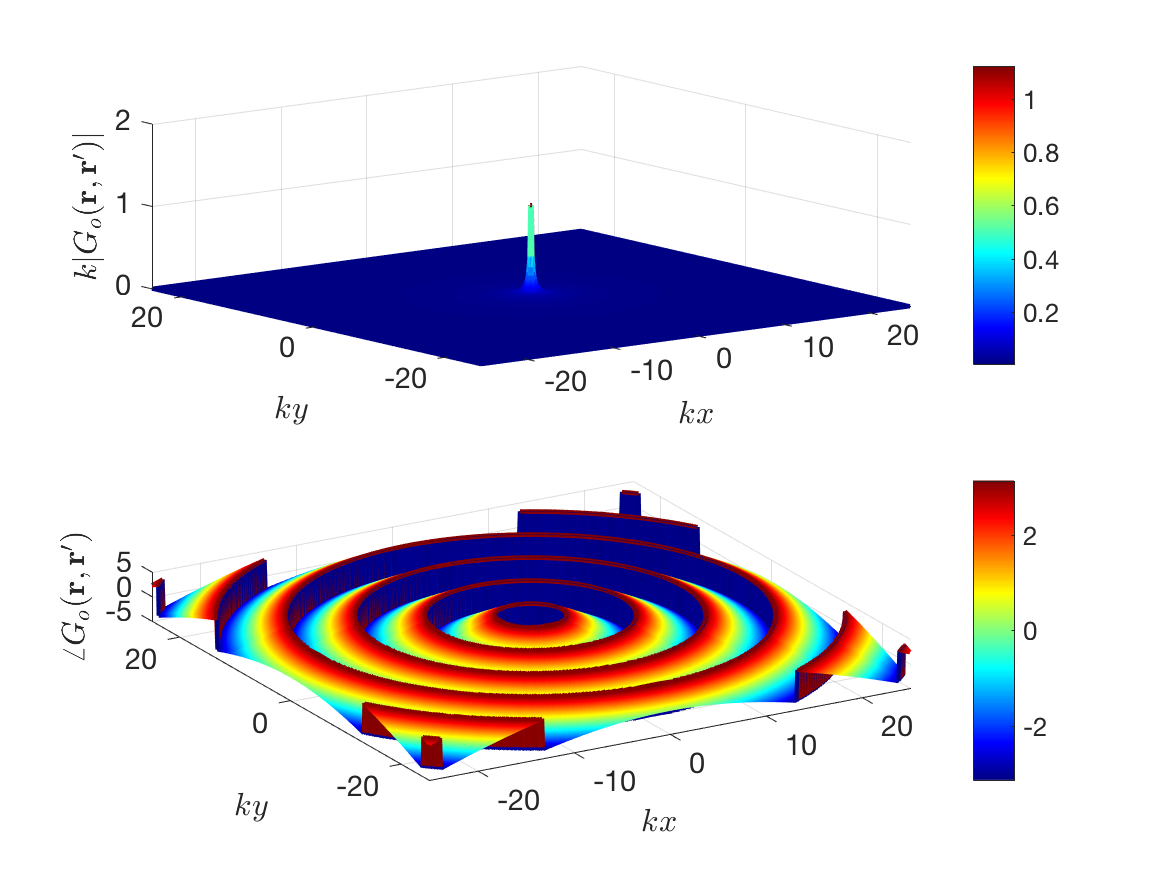
\includegraphics[width=4in]{../media/3d_fs_gf_mag.png}
\renewcommand{\baselinestretch}{1}
\small\normalsize
\begin{quote}
\caption[Magnitude and Phase of 3-D Free Space Green's Function]{ Magnitude and Phase of 3-D Free Space Green's Function\label{gf_fig:1}}
\end{quote}
\end{figure} 
\renewcommand{\baselinestretch}{2}
\small\normalsize

\begin{figure}[ht]
\centering
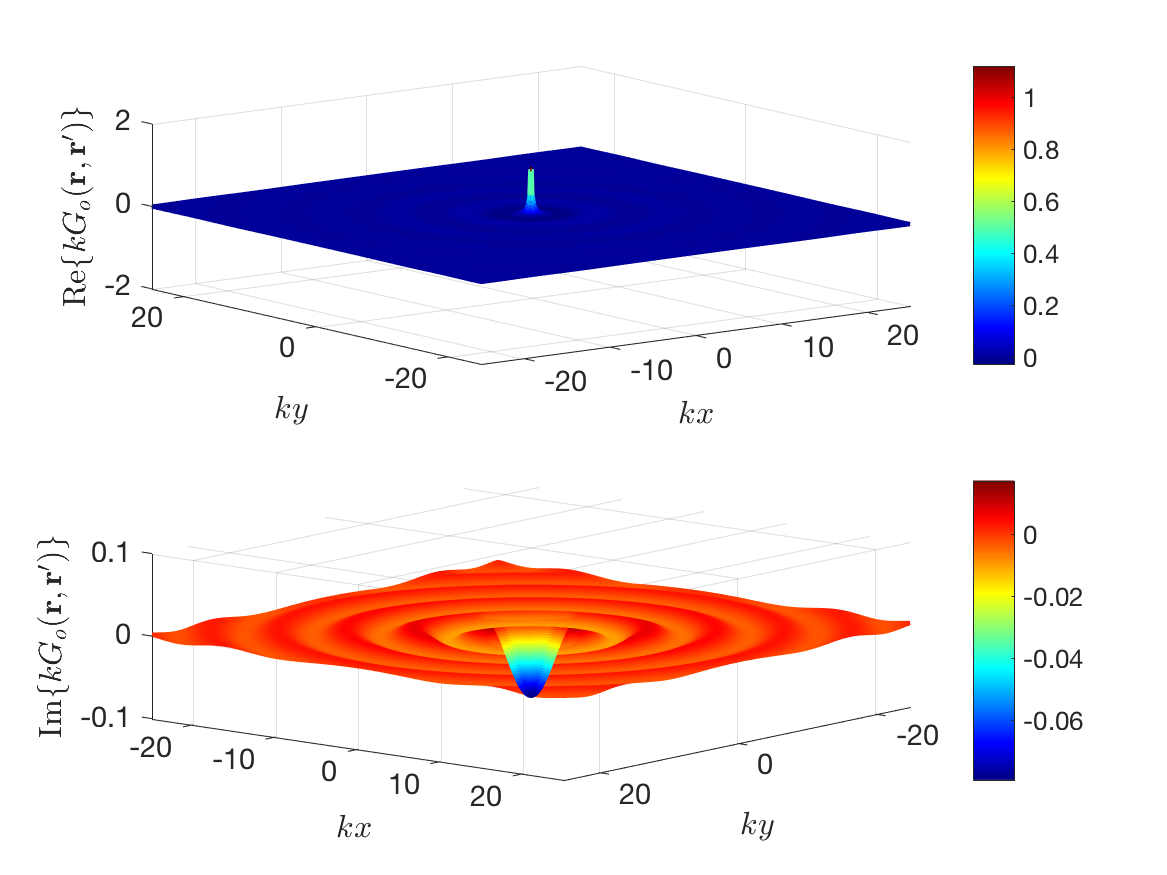
\includegraphics[width=4in]{../media/3d_fs_gf_re_im.png}
\renewcommand{\baselinestretch}{1}
\small\normalsize
\begin{quote}
\caption[Real and Imaginary Components of 3-D Free Space Green's Function]{Real and Imaginary Components of 3-D Free Space Green's Function \label{gf_fig:2}}
\end{quote}
\end{figure} 
\renewcommand{\baselinestretch}{2}
\small\normalsize

\subsubsection {Conversion to the Time Domain}
The Green's function in Equation \ref{gf_eq:26} is still in Fourier space. We can explicitly express the frequency dependence as:

\begin{equation}
G_o\left(\mathbf{r},\mathbf{r}',\omega\right) = \frac{e^{-j\frac{\omega n_r}{c}|\mathbf{r} - \mathbf{r}'|}}{4\pi |\mathbf{r} - \mathbf{r}'|}
\label{gf_eq:28}
\end{equation}
\renewcommand{\baselinestretch}{2} \small\normalsize

\noindent To determine the Green's function in the time domain, we need to take the inverse Fourier transform.

\begin{equation}
\begin{gathered}
G_o\left(\mathbf{r},\mathbf{r}',t\right) = \frac{1}{2\pi}\int\limits_{-\infty}^{\infty}d\omega e^{j\omega t}G_o\left(\mathbf{r},\mathbf{r}',\omega\right) \\
G_o\left(\mathbf{r},\mathbf{r}',t\right) = \frac{1}{2\pi}\int\limits_{-\infty}^{\infty}d\omega e^{j\omega t}  \frac{e^{-j\frac{\omega n_r}{c}|\mathbf{r}-\mathbf{r}'|}}{4\pi |\mathbf{r}-\mathbf{r}'|}\\
\end{gathered}
\label{gf_eq:29}
\end{equation}
\renewcommand{\baselinestretch}{2} \small\normalsize

\noindent Because the integration limits are $\pm\infty$, we can flip the sign in the exponential term.

\begin{equation}
\begin{gathered}
G_o\left(\mathbf{r},\mathbf{r}',t\right) = \frac{1}{4\pi |\mathbf{r}-\mathbf{r}'|}\frac{1}{2\pi}\int\limits_{-\infty}^{\infty}d\omega e^{-j\omega\left(\frac{n_r|\mathbf{r}-\mathbf{r}'|}{c} - t\right)} \\
G_o\left(\mathbf{r},\mathbf{r}',t\right) = \frac{1}{4\pi |\mathbf{r}-\mathbf{r}'|}\frac{1}{2\pi}\int\limits_{-\infty}^{\infty}d\omega e^{-j\omega\left(t - \frac{n_r|\mathbf{r}-\mathbf{r}'|}{c}\right)}
\end{gathered}
\label{gf_eq:29a}
\end{equation}
\renewcommand{\baselinestretch}{2} \small\normalsize

\noindent Recognizing that the Fourier transform of the delta function is:

\begin{equation}
\delta(t-t_0) = \frac{1}{2\pi}\int\limits_{-\infty}^{\infty}d\omega e^{-j\omega \left(t-t_0\right)}
\label{gf_eq:30}
\end{equation}
\renewcommand{\baselinestretch}{2} \small\normalsize

\noindent We can write the free space Green's function in the temporal domain as:

\begin{equation}
G_o\left(\mathbf{r},\mathbf{r}',t\right) = \frac{\delta\left(t-\frac{n_r|\mathbf{r}-\mathbf{r}'|}{c} \right)}{4\pi |\mathbf{r}-\mathbf{r}'|}
\label{gf_eq:31}
\end{equation}
\renewcommand{\baselinestretch}{2} \small\normalsize

Equation \ref{gf_eq:31} assumes the source is turned on at time $0$. If we let the source be turned on at an arbitrary time, $t'$, a more general expression is:

\begin{equation}
\boxed{G_o\left(\mathbf{r},\mathbf{r}',t,t'\right) = \frac{\delta\left(|t-t'|-\frac{n_r|\mathbf{r}-\mathbf{r}'|}{c} \right)}{4\pi |\mathbf{r}-\mathbf{r}'|}}
\label{gf_eq:32}
\end{equation}
\renewcommand{\baselinestretch}{2} \small\normalsize

In the time domain, we generally refer to $G_o\left(\mathbf{r},\mathbf{r}',t, t'\right)$ as the retarded wave solution because an observer will experience the source as if it acted at an earlier (retarded) time, $t_1=|t-t'|-n_r|\mathbf{r}-\mathbf{r}'|/c$.

\subsection {2-Dimensions}\label{gf_sec:2d}
This section derives the free space Green's function for the Helmholtz equation in 2-dimensional space. We will again work in the frequency domain first and then transform the result back to the time domain.

\subsubsection {Deriviation in the Frequency Domain}
In 2-dimensions,  rotational symmetry means that  $\partial G/\partial\phi =0$. Therefore we can expand the Laplacian of Equation \ref{gf_eq:19} in polar coordinates and neglect the $\phi$ components:

\begin{equation}
\frac{1}{\rho}\frac{\partial}{\partial \rho}\left(\rho\frac{\partial G}{\partial \rho}\right)+ k_o^2G = 0
\label{gf_eq:33}
\end{equation}
\renewcommand{\baselinestretch}{2} \small\normalsize

\noindent Equation \ref{gf_eq:33} is Bessel's equation with $\nu = 0$:

\begin{equation}
\frac{1}{\rho}\frac{\partial}{\partial \rho}\left(\rho\frac{\partial G}{\partial \rho}\right)+ \left(k_o^2 -\nu^2\right)G = 0
\label{gf_eq:34}
\end{equation}
\renewcommand{\baselinestretch}{2} \small\normalsize

\noindent The general solution to Equation \ref{gf_eq:33} is 

\begin{equation}
G = c_1J_0\left(k_o\rho\right) + c_2N_0\left(k_o\rho\right)
\label{gf_eq:35}
\end{equation}
\renewcommand{\baselinestretch}{2} \small\normalsize

Here $J_0$ is a Bessel function of the first kind, and $N_0$ is a Bessel function of the second kind. Since the delta function is singular at the origin, we can not demand that $G$ be finite at the origin. This means that $c_2 \neq 0$ and we have one equation with two unknowns.

When working with propagating waves, it is often more useful to work with Hankel functions than Bessel functions. The Hankel functions are defined as:

\begin{equation}
\begin{gathered}
H_0^{(1)}(k\rho) = J_0(k_o\rho) + jN_0(k_o\rho) \\
H_0^{(2)}(k\rho) = J_0(k_o\rho) - jN_0(k_o\rho)
\label{gf_eq:36}
\end{gathered}
\end{equation}
\renewcommand{\baselinestretch}{2} \small\normalsize

The Hankel functions behave asymptotically like waves as can be seen by their behavior for large arguments \cite{abramowitz_stegun}, which can be derived from the integral representation through the saddle point method as shown in Appendix \ref{appendix_saddle_point_method}.

\begin{equation}
\begin{gathered}
H_0^{(1)}(k_o\rho) \approx \sqrt{\frac{2}{\pi k_o\rho}}e^{j\left(k_o\rho - \frac{\pi}{4}\right)}\\
H_0^{(2)}(k_o\rho) \approx \sqrt{\frac{2}{\pi k_o\rho}}e^{-j\left(k_o\rho - \frac{\pi}{4}\right)}
\label{gf_eq:36a}
\end{gathered}
\end{equation}
\renewcommand{\baselinestretch}{2} \small\normalsize

We can now represent the solution to Equation \ref{gf_eq:33} in terms of Hankel functions as:

\begin{equation}
G = c_1H_0^{(1)}\left(k_o\rho\right) +c_2H_0^{(2)}\left(k_o\rho\right) 
\label{gf_eq:37}
\end{equation}
\renewcommand{\baselinestretch}{2} \small\normalsize

From the causality discussion in Section \ref{gf_sec:causality}, $H_0^{(2)}$ acts like an outward propagating wave while $H_0^{(1)}$ acts like an inward propagating wave. Therefore, $H_0^{(2)}$ is the physical solution, $c_1=0$, and the Green's function is:

\begin{equation}
G = c_2H_0^{(2)}\left(k_o\rho\right) 
\label{gf_eq:38}
\end{equation}
\renewcommand{\baselinestretch}{2} \small\normalsize

As in Section \ref{gf_sec:3d}, we integrate Equation \ref{gf_eq:9} over a small disk, $D$, centered at $\rho = 0$ and take the limit as $\rho \rightarrow 0$. For small arguments, the asymptotic behavior of $H_0^{(2)}(k_o\rho) \sim -j(2/\pi)\ln\left({k_o\rho}\right)$ and we can substitute $G = -j(2c_2/\pi)\ln\left({k_o\rho}\right)$ \cite{abramowitz_stegun}. 

\begin{equation}
\begin{gathered}
\lim_{\rho\to 0}\int\limits_{D} \left[ \frac{1}{\rho'}\frac{\partial}{\partial \rho'}\left(\rho' \frac{\partial G}{\partial \rho'} \right) + k_o^2G\right]\rho' d\rho' d\theta' = \lim_{\rho\to 0}\int\limits_{D} \delta\left(\boldsymbol{\rho}-\boldsymbol{\rho}' \right)\rho' d\rho' d\phi' \\
\lim_{\rho\to 0}\int\limits_{D} \left[ -\frac{1}{\rho'}\frac{\partial}{\partial \rho'}\left(\rho' jc_1\frac{2}{\pi}\frac{\partial \ln(k_o\rho')}{\partial \rho'} \right) - k_o^2jc_1\frac{2}{\pi}\ln(k_o\rho')\right]\rho' d\rho' d\theta' = -1 \\
\end{gathered}
\label{gf_eq:39}
\end{equation}
\renewcommand{\baselinestretch}{2} \small\normalsize

\noindent Integrating over $\theta'$ to get $2\pi$ and collecting the constants in the front yields:

\begin{equation}
\begin{gathered}
\lim_{\rho\to 0}-4jc_1\int\limits_{D} \left[\frac{\partial}{\partial \rho'}\left(\rho' \frac{\partial \ln(k_o\rho')}{\partial \rho'} \right) + k_o^2\rho'\ln(k_o\rho')\right] d\rho' = -1 \\
\lim_{\rho\to 0}4jc_1\left[\left(\rho' \frac{1 }{\rho'} \right)\bigg|_0^{\rho} + \int\limits_{D}k_o^2\rho'\ln(k_o\rho') d\rho'\right] = 1 \\
\end{gathered}
\label{gf_eq:39a}
\end{equation}
\renewcommand{\baselinestretch}{2} \small\normalsize

\noindent Integrating the second term by parts results in the following:

\begin{equation}
\begin{gathered}
\lim_{\rho\to 0}c_1\left[ 1 +  k_o^2\left( \ln(k_o\rho')\frac{\rho'^2}{2}\bigg|_0^{\rho} - \int\limits_{D}\frac{\rho'^2}{2}\frac{1}{\rho'} d\rho' \right)\right] = -\frac{j}{4} \\
\lim_{\rho\to 0}c_1\left[ 1 +  k_o^2\left( \ln(k_o\rho)\frac{\rho^2}{2} - \frac{1}{2}\int\limits_{D}\rho' d\rho' \right)\right] = -\frac{j}{4} \\
\end{gathered}
\label{gf_eq:39c}
\end{equation}
\renewcommand{\baselinestretch}{2} \small\normalsize

\noindent Finally we can simplify the result.

\begin{equation}
\begin{gathered}
\lim_{\rho\to 0}c_1\left[ 1 - \frac{\rho^2}{4}\right] = \frac{j}{4} \\
c_1 = -\frac{j}{4}\\
\end{gathered}
\label{gf_eq:39d}
\end{equation}
\renewcommand{\baselinestretch}{2} \small\normalsize

Now letting $\rho \rightarrow |\boldsymbol{\rho}-\boldsymbol{\rho}'|$, we have the final free space 2-dimensional Green's function, $G_o$:

\begin{equation}
\boxed{G_o\left(\boldsymbol{\rho},\boldsymbol{\rho}'\right) = -\frac{j}{4}H_0^{(2)}\left(k_o|\boldsymbol{\rho} - \boldsymbol{\rho}' | \right)}
\label{gf_eq:40}
\end{equation}
\renewcommand{\baselinestretch}{2} \small\normalsize

To help visualize this Green's function, the magnitude and phase are shown in Figure \ref{gf_fig:3} and the real and imaginary components are shown in Figure \ref{gf_fig:4}.

\begin{figure}[ht]
\centering
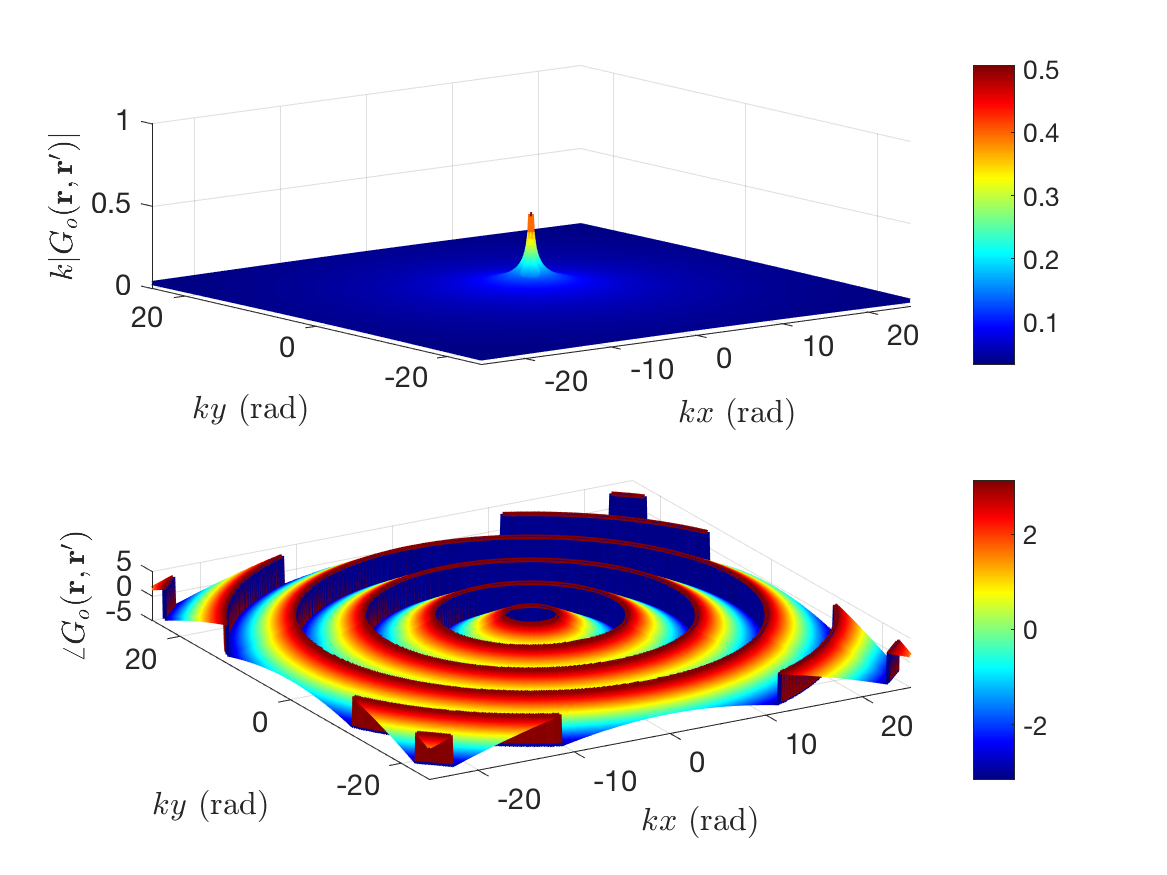
\includegraphics[width=4in]{../media/2d_fs_gf_mag.png}
\renewcommand{\baselinestretch}{1}
\small\normalsize
\begin{quote}
\caption[Magnitude and Phase of 2-D Free Space Green's Function]{Magnitude and Phase of 2-D Free Space Green's Function \label{gf_fig:3}}
\end{quote}
\end{figure} 
\renewcommand{\baselinestretch}{2}
\small\normalsize

\begin{figure}[ht]
\centering
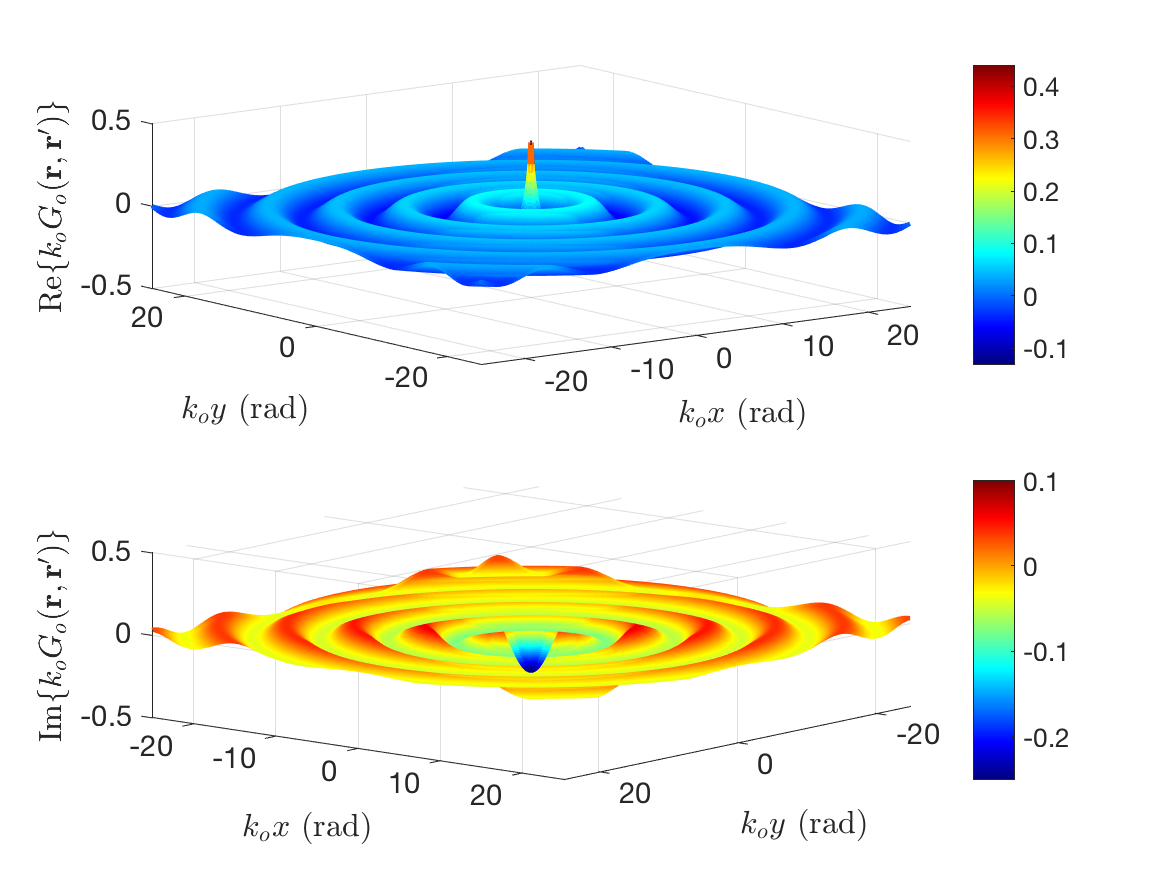
\includegraphics[width=4in]{../media/2d_fs_gf_re_im.png}
\renewcommand{\baselinestretch}{1}
\small\normalsize
\begin{quote}
\caption[Real and Imaginary Components of 2-D Free Space Green's Function]{Real and Imaginary Components of 2-D Free Space Green's Function \label{gf_fig:4}}
\end{quote}
\end{figure} 
\renewcommand{\baselinestretch}{2}
\small\normalsize

\subsubsection {Conversion to the Time Domain}
As in Section \ref{gf_sec:3d}, the Green's function in Equation \ref{gf_eq:40} is still in Fourier space. We can explicitly express the frequency dependence as:

\begin{equation}
G_o\left(\boldsymbol{\rho},\boldsymbol{\rho}',\omega\right) = -\frac{j}{4}H_0^{(2)}\left(\frac{\omega n_r}{c}|\boldsymbol{\rho} - \boldsymbol{\rho}' | \right)
\label{gf_eq:40a}
\end{equation}
\renewcommand{\baselinestretch}{2} \small\normalsize

To determine the Green's function in the time domain, we need to take the inverse Fourier transform and will follow the procedure outlined in \cite{gbur_math}.

\begin{equation}
\begin{gathered}
G_o\left(\boldsymbol{\rho},\boldsymbol{\rho}',t\right) = \frac{1}{2\pi}\int\limits_{-\infty}^{\infty}d\omega e^{j\omega t}G_o\left(\boldsymbol{\rho},\boldsymbol{\rho}',\omega\right) \\
G_o\left(\boldsymbol{\rho},\boldsymbol{\rho}',t\right) = -\frac{j}{4}\frac{1}{2\pi}\int\limits_{-\infty}^{\infty}d\omega e^{j\omega t} H_0^{(2)}\left(\frac{\omega n_r}{c}|\boldsymbol{\rho} - \boldsymbol{\rho}' | \right)\\
\end{gathered}
\label{gf_eq:40b}
\end{equation}
\renewcommand{\baselinestretch}{2} \small\normalsize

We can use a representation of $H_0^{(2)}$ that is related to the Mehler-Sonine integral representation \cite{nist_handbook}:

\begin{equation}
H_o^{(2)}\left(z\right) = -\frac{1}{j\pi}\int\limits_{-\infty}^{\infty}e^{-jz\cosh(\tau)}d\tau = -\frac{2}{j\pi}\int\limits_{0}^{\infty}e^{-jz\cosh(\tau)}d\tau
\label{gf_eq:40c}
\end{equation}
\renewcommand{\baselinestretch}{2} \small\normalsize

\noindent Equation \ref{gf_eq:40c} is valid for $z>0$ . Since $k_o| \boldsymbol{\rho} - \boldsymbol{\rho}'| > 0$, this condition is satisfied. Letting $\rho' \rightarrow 0$ for simplification yields:

\begin{equation}
G_o\left(\boldsymbol{\rho},0,t\right) = \frac{1}{4\pi^2}\int\limits_{-\infty}^{\infty}d\omega e^{j\omega t} \int\limits_{0}^{\infty}e^{-j\frac{\omega n_r}{c}\rho\cosh(\tau)}d\tau\\
\label{gf_eq:40d}
\end{equation}
\renewcommand{\baselinestretch}{2} \small\normalsize

\noindent We can bring the integral over $\omega$ inside the integral over $\tau$.

\begin{equation}
\begin{gathered}
G_o\left(\boldsymbol{\rho},0,t\right) = \frac{1}{4\pi^2}\int\limits_{0}^{\infty}d\tau\int\limits_{-\infty}^{\infty}d\omega e^{j\omega t} e^{-j\frac{\omega n_r}{c}\rho\cosh(\tau)}\\
G_o\left(\boldsymbol{\rho},0,t\right) = \frac{1}{4\pi^2}\int\limits_{0}^{\infty}d\tau\int\limits_{-\infty}^{\infty}d\omega e^{-j\omega \left(\frac{n_r\rho \cosh(\tau)}{c} - t\right)}\\
G_o\left(\boldsymbol{\rho},0,t\right) = \frac{1}{4\pi^2}\int\limits_{0}^{\infty}d\tau\int\limits_{-\infty}^{\infty}d\omega e^{-j\omega \left(t - \frac{n_r\rho \cosh(\tau)}{c}\right)}\\
\end{gathered}
\label{gf_eq:40e}
\end{equation}
\renewcommand{\baselinestretch}{2} \small\normalsize

\noindent Again using the definition of the delta function from Equation \ref{gf_eq:30} yields:

\begin{equation}
G_o\left(\boldsymbol{\rho},0,t\right) = \frac{1}{2\pi}\int\limits_{0}^{\infty}d\tau \delta\left(t - \frac{n_r\rho \cosh(\tau)}{c}\right)\\
\label{gf_eq:40f}
\end{equation}
\renewcommand{\baselinestretch}{2} \small\normalsize

For $G_o\left(\boldsymbol{\rho},0,t\right)$ to be nonzero, $t - n_r\rho \cosh(\tau)/c > 0$ for all values of $\tau$. This means $t > n_r\rho/c$ and we can enforce this condition on $t$ through the Heaviside step function, $H\left(t -n_r\rho/c\right)$:

 \begin{equation}
G_o\left(\boldsymbol{\rho},0,t\right) = \frac{1}{2\pi}\int\limits_{0}^{\infty}d\tau H\left(t -\frac{n_r\rho}{c}\right) \delta\left(t - \frac{n_r\rho \cosh(\tau)}{c}\right)
\label{gf_eq:40g}
\end{equation}
 \renewcommand{\baselinestretch}{2} \small\normalsize
 
Because the argument of the delta function is a complicated function of $t$, we need to use the composition property of the delta function \cite{arfken_weber}, \cite{gbur_math}.

 \begin{equation}
\delta\left(g(x) \right) = \sum_{\substack{a \\g(a)=0}}\frac{\delta(x-a)}{|g'(a)|}
\label{gf_eq:40h}
\end{equation}
 \renewcommand{\baselinestretch}{2} \small\normalsize
 
From Equation \ref{gf_eq:40g}, $g(\tau) = t - n_r\rho\cosh(\tau)/c$ and the only zero  is $\tau = \cosh^{-1}\left(ct/n_r\rho\right)$. We can now rewrite the delta function from Equation \ref{gf_eq:40g} as:

 \begin{equation}
\delta\left(t - \frac{n_r\rho \cosh(\tau)}{c}\right) = \frac{\delta\left(\tau -\cosh^{-1}\left(\frac{ct}{n_r\rho} \right) \right)}{n_r\rho\sinh\left(\cosh^{-1}\left(\frac{ct}{n_r\rho} \right) \right)}
\label{gf_eq:40i}
\end{equation}
 \renewcommand{\baselinestretch}{2} \small\normalsize
 
\noindent We can now rewrite Equation \ref{gf_eq:40g} as:

 \begin{equation}
 \begin{gathered}
G_o\left(\boldsymbol{\rho},0,t\right) = \frac{1}{2\pi}\int\limits_{0}^{\infty}d\tau H\left(t -\frac{n_r\rho}{c}\right)  \frac{c\delta\left(\tau -\cosh^{-1}\left(\frac{ct}{n_r\rho} \right) \right)}{n_r\rho\sinh\left(\cosh^{-1}\left(\frac{ct}{n_r\rho} \right) \right)}\\
G_o\left(\boldsymbol{\rho},0,t\right) = \frac{cH\left(t -\frac{n_r\rho}{c}\right)}{2\pi n_r\rho\sinh\left(\cosh^{-1}\left(\frac{ct}{n_r\rho} \right) \right)}\int\limits_{0}^{\infty}d\tau \delta\left(\tau -\cosh^{-1}\left(\frac{ct}{n_r\rho} \right) \right)\\
G_o\left(\boldsymbol{\rho},0,t\right) = \frac{cH\left(t -\frac{n_r\rho}{c}\right)}{2\pi n_r\rho\sinh\left(\cosh^{-1}\left(\frac{ct}{n_r\rho} \right) \right)}
\end{gathered}
\label{gf_eq:40j}
\end{equation}
 \renewcommand{\baselinestretch}{2} \small\normalsize
 
\noindent Using the identity that $\sinh\left(\cosh^{-1}(x) \right) = \sqrt{x^2 -1}$:

 \begin{equation}
 \begin{gathered}
G_o\left(\boldsymbol{\rho},0,t\right) = \frac{cH\left(t -\frac{n_r\rho}{c}\right)}{2\pi n_r\rho\sqrt{\left(\frac{ct}{n_r\rho} \right)^2 - 1}     }\\
G_o\left(\boldsymbol{\rho},0,t\right) = \frac{H\left(t -n_r\frac{\rho}{c}\right)}{2\pi \sqrt{t^2 - \left(\frac{n_r\rho}{c}\right)^2}     }
\end{gathered}
\label{gf_eq:40k}
\end{equation}
 \renewcommand{\baselinestretch}{2} \small\normalsize
 
\noindent Letting $t\rightarrow |t-t'|$ and $\rho \rightarrow |\boldsymbol{\rho} - \boldsymbol{\rho}'|$ yields the final result:

 \begin{equation}
\boxed{G_o\left(\boldsymbol{\rho},\boldsymbol{\rho}',t,t'\right) = \frac{H\left(|t-t'| -\frac{n_r|\boldsymbol{\rho} - \boldsymbol{\rho}'|}{c}\right)}{2\pi \sqrt{|t-t'|^2 -\left(\frac{n_r|\boldsymbol{\rho} - \boldsymbol{\rho}'|}{c}\right)^2 }     }}
\label{gf_eq:40l}
\end{equation}
\renewcommand{\baselinestretch}{2} \small\normalsize

\subsection {Paraxial Wave Equation} \label{gf_sec:paraxial}
In this section we derive the Green's function for the paraxial wave equation in the frequency domain.

\subsubsection {Derivation of the Paraxial Wave Equation}
We can derive the paraxial from the Helmholtz equation by assuming a wave propagating in the $x$ direction and allow the amplitude to vary slowly in all directions. We will introduce the freespace wave number, $k_p = \omega /c$ to keep the index of refraction explicitly separate so that our scalar wave takes the form $U(x,z) = A(x,z)e^{-jk_px}$. We will see that with this assumption, the Green's function dependence on the index of refraction is factored out into a phase term.

 \begin{equation}
 \begin{gathered}
 \left[ \nabla^2 + k_p^2n_r^2\right]U = 0 \\
\left[\frac{\partial^2 }{\partial x^2} + \frac{\partial^2 }{\partial z^2} + k_p^2n_r^2\right]U = 0 \\
\frac{\partial }{\partial x}\left(\frac{\partial U}{\partial x} \right) + \frac{\partial^2 U}{\partial z^2} + k_p^2n_r^2 U = 0 \\
\end{gathered}
\label{gf_eq:41}
\end{equation}
\renewcommand{\baselinestretch}{2} \small\normalsize

\noindent Expanding the derivative in terms of $x$ yields the following:

 \begin{equation}
 \begin{gathered}
\frac{\partial }{\partial x}\left(-jk_pAe^{-jk_px}+e^{-jk_px}\frac{\partial A}{\partial x} \right) + e^{-jk_px}\frac{\partial^2 A}{\partial z^2} + k_p^2n_r^2 Ae^{-jk_px} = 0 \\
-k_p^2Ae^{-jk_px} -2jk_pe^{-jk_px}\frac{\partial A}{\partial x}+e^{-jk_px}\frac{\partial^2 A}{\partial x^2} + e^{-jk_px}\frac{\partial^2 A}{\partial z^2} + k_p^2n_r^2 Ae^{-jk_px} = 0 \\
e^{-jk_px}\left[ -2jk_p\frac{\partial A}{\partial x}+\frac{\partial^2 A}{\partial x^2} + \frac{\partial^2 A}{\partial z^2} + k_p^2\left(n_r^2-1\right)A\right] = 0 \\
\end{gathered}
\label{gf_eq:41a}
\end{equation}
\renewcommand{\baselinestretch}{2} \small\normalsize
 
\noindent This gives us an equation dependent only on the amplitude, $A$

 \begin{equation}
-2jk_p\frac{\partial A}{\partial x}+\frac{\partial^2 A}{\partial x^2} + \frac{\partial^2 A}{\partial z^2} + k_p^2\left(n_r^2-1\right)A= 0 \\
\label{gf_eq:42}
\end{equation}
 \renewcommand{\baselinestretch}{2} \small\normalsize
 
We can now apply the paraxial approximation which is that the change in the modulation function along the propagation direction is negligible over a wavelength. This can be expressed mathematically as:
 
  \begin{equation}
k_p\frac{\partial A}{\partial x} >> \frac{\partial^2 A}{\partial^2 x}
\label{gf_eq:43}
\end{equation}
 \renewcommand{\baselinestretch}{2} \small\normalsize
 
With this approximation we can neglect the 2nd derivative in $x$ and write the paraxial equation as
 
\begin{equation}
\boxed{-2jk_p\frac{\partial A}{\partial x} + \frac{\partial^2 A}{\partial z^2} +k_p^2\left(n_r^2-1\right)A= 0} \\
\label{gf_eq:44}
\end{equation}
\renewcommand{\baselinestretch}{2} \small\normalsize
 
The paraxial wave equation is a parabolic differential equation with the same structure as the diffusion equation. However, since the effective diffusion coefficient is complex, we can expect the solution to oscillate rather than decay exponentially. Since we have reduced the original Helmholtz equation for the full propagating wave to one that is only dependent on the modulation function, we will need to scale the Green's function by $e^{-jk_px}$ to get the full propagating wave solution.
 
\subsubsection {Green's Function Derivation in the Frequency Domain} \label{gf_sec:paraxial_gf_derivation}
As stated in the previous section, the Green's function for the paraxial wave equation, $G_p$, will only define the amplitude modulation. To get the full Green's function, we will need to scale by the plane wave, $G_o= G_p e^{-jk_px}$. We can start with substituting the Greens function into equation \ref{gf_eq:44}.

\begin{equation}
-2jk_p\frac{\partial G_p}{\partial x} + \frac{\partial^2 G_p}{\partial z^2} +k_p^2(n_r^2-1)\hat{G_p}= -\delta(x)\delta(z)
\label{gf_eq:44a}
\end{equation}
 \renewcommand{\baselinestretch}{2} \small\normalsize
 
We can then take the Fourier transform of Equation \ref{gf_eq:44a} along $z$ and multiply both sides by $-1$.

\begin{equation}
2jk_p\frac{\partial \hat{G_p}}{\partial x} +k^2\hat{G_p} -k_p^2(n_r^2-1)\hat{G_p}= \delta(x)
\label{gf_eq:45}
\end{equation}
 \renewcommand{\baselinestretch}{2} \small\normalsize
 
Solving away from the delta function yields the following expression for $\hat{G_p}$:

\begin{equation}
\begin{aligned}
\hat{G_p}&=c\exp\left[-\frac{k^2 - k_p^2(n_r^2-1)}{2jk_p}x \right]\\
&= c\exp\left[\frac{jk^2}{2k_p}x \right] \exp\left[-\frac{jk_p(n_r^2-1)}{2}x\right]
\end{aligned}
\label{gf_eq:46}
\end{equation}
 \renewcommand{\baselinestretch}{2} \small\normalsize
 
Here we see that the dependence on the index of refraction is separated into a phase term that is independent of $k$. To find $c$, we can integrate Equation \ref{gf_eq:45} over a small region $\pm\epsilon$ and take the limit as $x\rightarrow 0$.

\begin{equation}
\lim_{x\rightarrow 0}\int_{-\epsilon}^{\epsilon}dx\left[2jk_p\frac{\partial\hat{G_p}}{\partial x}+ k^2\hat{G_p} -k_p^2(n_r^2-1)\hat{G_p} \right] = \lim_{x\rightarrow 0}\int_{-\epsilon}^{\epsilon}dx\delta(x)\\
\label{gf_eq:47}
\end{equation}
 \renewcommand{\baselinestretch}{2} \small\normalsize
 
\noindent $\hat{G_p}$ must be continuous, so the integral over the $k^2\hat{G_p}$ and $k_p^2(n_r^2-1)\hat{G_p}$ terms must be 0.

\begin{equation}
\begin{gathered}
\lim_{x\rightarrow 0}2jk_p\int_{-\epsilon}^{\epsilon}dx\frac{\partial\hat{G_p}}{\partial x}= 1\\
\lim_{x\rightarrow 0}2jk_p\hat{G_p} = 1 \\
\lim_{x\rightarrow 0}2jk_pc\exp\left[\frac{jk^2}{2k_p}x\right]\exp\left[\frac{-jk_p(n_r^2-1)}{2}x\right] = 1\\
c = \frac{1}{j2k_p}\\
\end{gathered}
\label{gf_eq:11cb}
\end{equation}
 \renewcommand{\baselinestretch}{2} \small\normalsize
 
\noindent This yields the final expression for $\hat{G_p}$:

\begin{equation}
\hat{G_p}= \frac{1}{2jk_p}e^{\frac{jk^2}{2k_p}x}e^{\frac{-jk_p(n_r^2-1)}{2}x}
\label{gf_eq:11cc}
\end{equation}
 \renewcommand{\baselinestretch}{2} \small\normalsize
 
\noindent To find $G_p$, we can take the inverse Fourier transform of $\hat{G_p}$:

\begin{equation}
\begin{aligned}
G_p &= \mathcal{F}^{-1}\{\hat{G_p}\} = \frac{1}{2jk_p}\frac{1}{2\pi}\int_{-\infty}^{\infty}dk e^{\frac{jk^2}{2k_p}x}e^{-\frac{jk_p(n_r^2-1)}{2}x}e^{-jkz} \\
& = \frac{1}{2jk_p}\frac{1}{2\pi}e^{-\frac{jk_p(n_r^2-1)}{2}x}\int_{-\infty}^{\infty}dk e^{\frac{jk^2}{2k_p}x-jkz} \\
\end{aligned}
\label{gf_eq:11d}
\end{equation}
 \renewcommand{\baselinestretch}{2} \small\normalsize
 
\noindent To solve this, we need to complete the square with respect to $k$

\begin{equation}
\begin{gathered}
\frac{jx}{2k_p}\left[k^2  -2k\frac{k_pz}{x}\right]\\
\frac{jx}{2k_p}\left[\left(k - \frac{k_pz}{x}\right)^2 - \frac{k_p^2z^2}{x^2} \right]\\
\frac{jx}{2k_p}\left(k - \frac{k_pz}{x}\right)^2 - \frac{jk_pz^2}{x}\\
\end{gathered}
\label{gf_eq:11e}
\end{equation}
 \renewcommand{\baselinestretch}{2} \small\normalsize
 
\noindent Now we can substitute into Equation \ref{gf_eq:11d}

\begin{equation}
\begin{aligned}
G_p &= \frac{1}{2jk_p}\frac{1}{2\pi}e^{-\frac{jk_p(n_r^2-1)}{2}x}\int_{-\infty}^{\infty}dk e^{\frac{jx}{2k_p}\left(k  -\frac{k_pz}{x}\right)^2- \frac{jk_p}{2x}z^2 } \\
&= \frac{1}{2jk_p}\frac{1}{2\pi} \sqrt{\frac{\pi j2k_p}{x}}e^{-\frac{jk_p(n_r^2-1)}{2}x}e^{-j\frac{k_p}{2x}z^2 } \\
\end{aligned}
\label{gf_eq:11f}
\end{equation}
 \renewcommand{\baselinestretch}{2} \small\normalsize
 
\noindent Collecting terms and simplifying yields the following.

 \begin{equation}
\begin{aligned}
G_p &= \frac{1}{2jk_p}\sqrt{\frac{jk_p}{2\pi x}}\exp\left[\frac{-jk_p(n_r^2-1)}{2}x\right]\exp\left[-j\frac{k_pz^2}{2x} \right]\\
&= \sqrt{\frac{1}{8\pi j k_px}}\exp\left[\frac{-jk_p(n_r^2-1)}{2}x\right]\exp\left[-j\frac{k_pz^2}{2x} \right]\\
\end{aligned}
\label{gf_eq:11ffa}
\end{equation}
 \renewcommand{\baselinestretch}{2} \small\normalsize
 
\noindent Multiplying by $e^{-jk_px}$ yields the full Green's function.

\begin{equation}
G_o= \sqrt{\frac{1}{8\pi jk_px}}\exp\left[-\frac{jk_p(n_r^2-1)}{2}x\right]\exp\left[-j\frac{k_pz^2}{2x} \right]e^{-jk_px}
\label{gf_eq:11fa}
\end{equation}
  \renewcommand{\baselinestretch}{2} \small\normalsize
  
We can let $x\rightarrow |x-x'|$, $x\rightarrow |z-z'|$ and introduce the modified refractivity, $m = n_r^2-1$ to present the final version of the Green's function.

\begin{equation}
\boxed{G_o\left(x,x',z,z' \right)= \sqrt{\frac{1}{8\pi jk_p|x-x'|}}\exp\left[-jk_p\left(|x-x'|\left[1+\frac{m}{2}\right] + \frac{|z-z'|^2}{2|x-x'|}\right)\right]}\\
\label{gf_eq:11fb}
\end{equation}
 \renewcommand{\baselinestretch}{2} \small\normalsize
 
To help visualize this Green's function, the magnitude and phase is shown in Figure \ref{gf_fig:5} and the real and imaginary components are shown in Figure \ref{gf_fig:6}. Both figures show a slice of the Green's function along $z = 0$. 

\begin{figure}[ht]
\centering
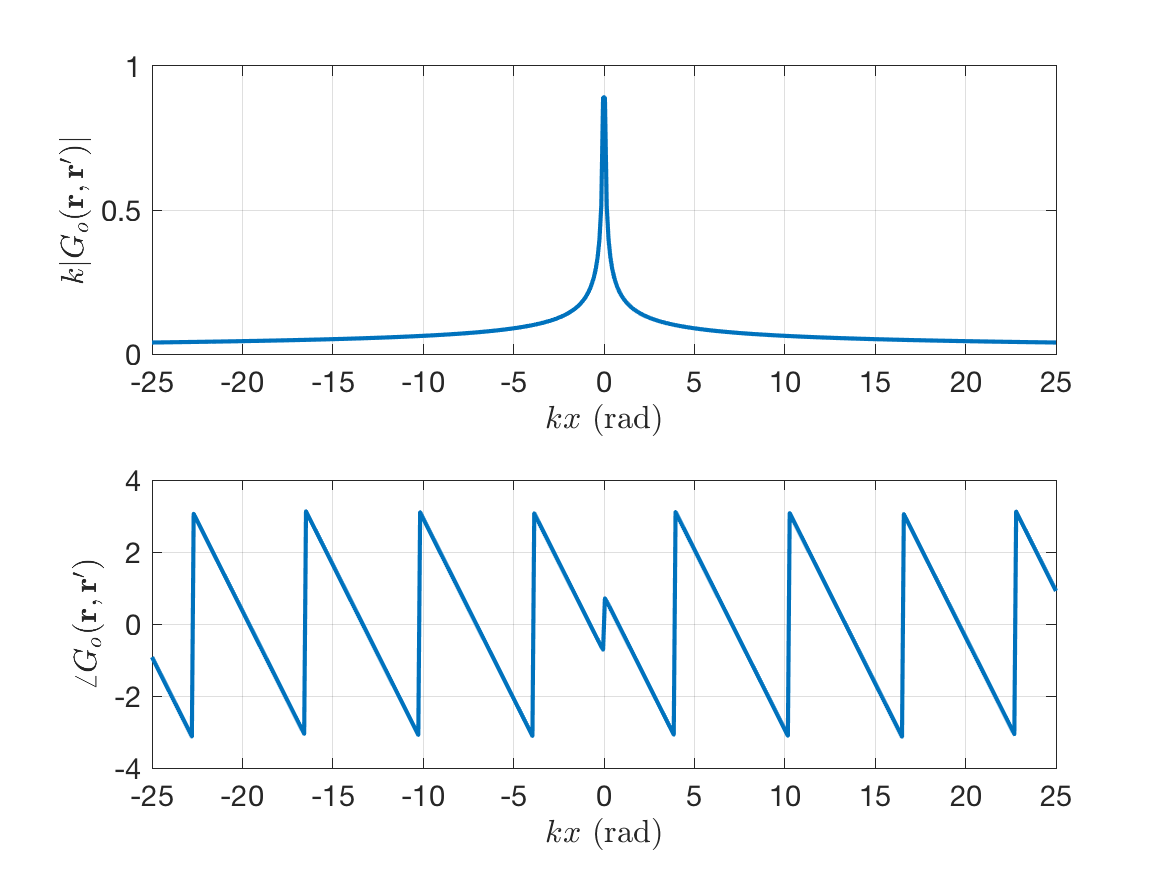
\includegraphics[width=4in]{../media/2d_paraxial_gf_mag.png}

\renewcommand{\baselinestretch}{1}
\small\normalsize
\begin{quote}
\caption[Magnitude and Phase of 2-D Paraxial Green's Function]{Magnitude and Phase of 2-D Paraxial Green's Function \label{gf_fig:5}}
\end{quote}
\end{figure} 
\renewcommand{\baselinestretch}{2}
\small\normalsize

\begin{figure}[ht]
\centering
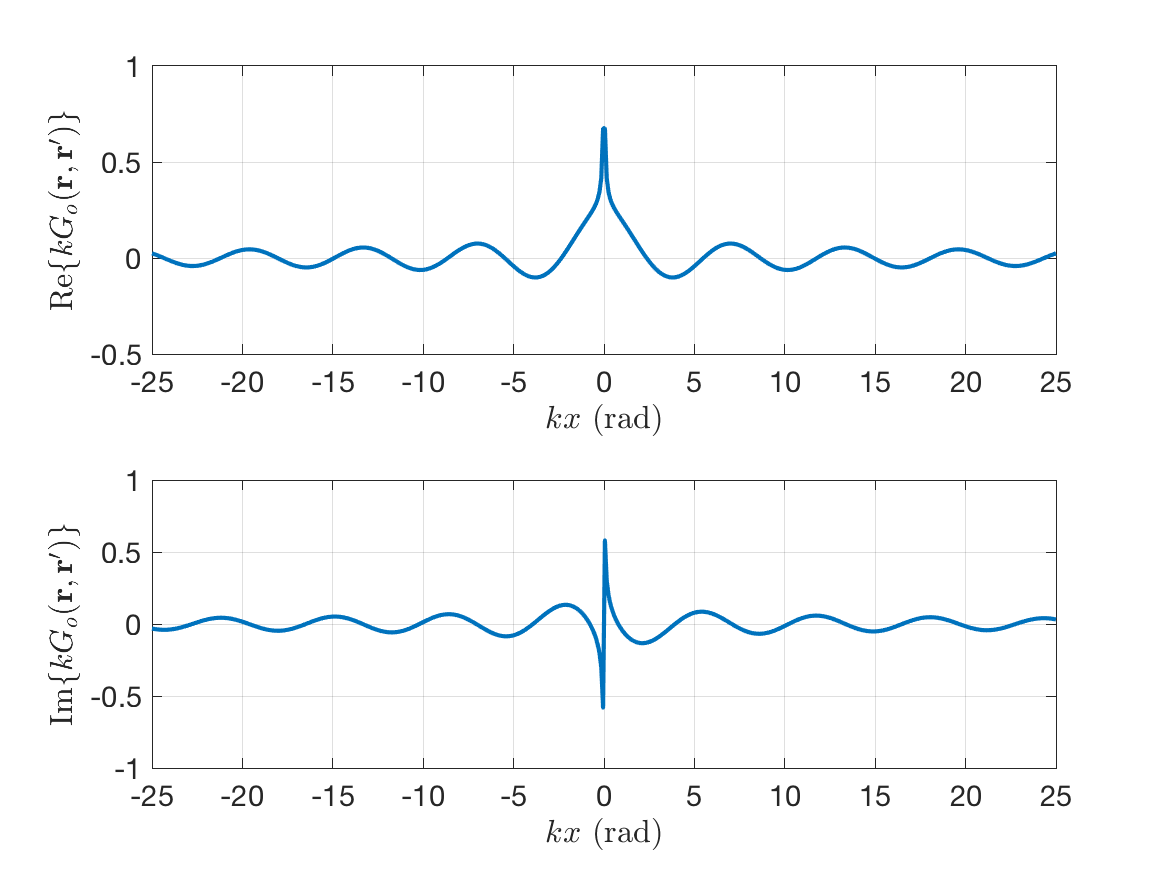
\includegraphics[width=4in]{../media/2d_paraxial_gf_re_im.png}

\renewcommand{\baselinestretch}{1}
\small\normalsize
\begin{quote}
\caption[Real and Imaginary Components of 2-D Paraxial Green's Function]{Real and Imaginary Components of 2-D Paraxial Green's Function \label{gf_fig:6}}
\end{quote}
\end{figure} 
\renewcommand{\baselinestretch}{2}
\small\normalsize

It is important to note that with the paraxial approximation, only forward propagating waves are included in the solution, which will become more apparent when we discuss the parabolic wave equation. This means that effects such as backscattering are not captured with this method. 

\subsubsection{Derivation From 3-D Free Space Green's Function}
A simpler method to derive the Green's function for the paraxial wave equation is to apply the paraxial assumption to the 3-D free space Green's function. This assumption allows us to substitute $r$ with $x$ for the amplitude, but we will need to integrate out the $y$ dependence of the phase because it is rapidly oscillating. We can use a binomial expansion to separate the $y$ and $z$ dependence.

\begin{equation}
r = \sqrt{x^2+y^2+z^2} \approx x + \frac{y^2}{2x}+\frac{z^2}{2x}
\label{gf_eq:11za}
\end{equation}
 \renewcommand{\baselinestretch}{2} \small\normalsize
 
\noindent The paraxial approximation of the 3-D free space Green's function is then

\begin{equation}
G_o \approx \frac{\exp\left[-jk_o\left(x+\frac{z^2}{2x} \right)\right]}{4\pi x} \exp\left[-jk_o\frac{y^2}{2x}\right]
\label{gf_eq:11zb}
\end{equation}
 \renewcommand{\baselinestretch}{2} \small\normalsize
 
\noindent We can integrate out the $y$ dependence

\begin{equation}
\int_{-\infty}^{\infty} dy \exp\left[-jk_o\frac{y^2}{2x}\right] = \sqrt{\frac{2\pi x}{jk_o}}
\label{gf_eq:11zc}
\end{equation}
 \renewcommand{\baselinestretch}{2} \small\normalsize
 
\noindent Substituting back into Equation \ref{gf_eq:11zb}

\begin{equation}
\begin{aligned}
G_o &= \frac{\exp\left[-jk_o\left(x+\frac{z^2}{2x} \right)\right]}{4\pi x} \sqrt{\frac{2\pi x}{jk_o}}\\
&= \sqrt{\frac{1}{j8\pi k_o x}}\exp\left[-jk_o\left(x+\frac{z^2}{2x} \right)\right]
\label{gf_eq:11zd}
\end{aligned}
\end{equation}
 \renewcommand{\baselinestretch}{2} \small\normalsize
 
Equation \ref{gf_eq:11zd} is different from Equation  \ref{gf_eq:11fa} in that the dependence on the index of refraction is no longer separable into a phase term. This is however the same answer we would have gotten if we assumed the propagating wave had the form $U(x,z) = A(x,z)e^{-jk_ox}$ when deriving the paraxial wave equation. If we let $n_r = 1$, then these two equations will be identical.

\subsection{Parabolic Wave Equation}
This section derives the Green's function for the parabolic wave equation (PWE), which is essentially the paraxial wave equation with a correction factor to account for the curvature of the earth.

\subsubsection{Earth Flattening Transformation}
Because the earth is actually curved and not flat, it is often useful to treat the earth as a sphere when analyzing propagation. If we let $a_e$ be the radius of the earth, we can use a conformal mapping to implement the transformation \cite{kuttler_pe_theory} and keep the result in Cartesian coordinates.

\begin{equation}
\begin{gathered} 
\xi = 2a_e\frac{a_e+j\zeta}{\zeta + ja_e} \\
\zeta = r\sin(\theta) + jr\cos(\theta)  \quad \xi=x+jz\\
\label{gf_eq:74}
\end{gathered}
\end{equation}
\renewcommand{\baselinestretch}{2} \small\normalsize

Using this mapping and applying the paraxial approximation to the Helmholtz equation with refractivity included yields the PWE \cite{kuttler_pe_theory} \cite{dockery_pe}.
 
\begin{equation}
-2jk_p\frac{\partial A}{\partial x} + \frac{\partial^2 A}{\partial z^2} +k_p^2\left(n^2-1+\frac{2z}{a_e} \right)A = 0 \\
\label{gf_eq:75}
\end{equation}
\renewcommand{\baselinestretch}{2} \small\normalsize

The only difference between Equation \ref{gf_eq:75} and Equation \ref{gf_eq:44} is the inclusion of the term $2z/a_e$ that represents the impact of the curvature of the Earth. We can incorporate this correction factor in the modified refractivity, $m_z = n^2-1 + 2z/a_e = m + 2z/a_e$, and treat it as a constant in $z$. With this substitution, we are explicitly defining the PWE as a special case of the paraxial wave equation that includes a correction factor for the curvature of the earth.

\begin{equation}
-2jk_p\frac{\partial A}{\partial x} + \frac{\partial^2 A}{\partial z^2} +k_p^2m_zA = 0 \\
\label{gf_eq:76}
\end{equation}
\renewcommand{\baselinestretch}{2} \small\normalsize

\subsubsection{Factorization of the Helmholtz Equation}
Equation \ref{gf_eq:76} is sometimes referred to as the narrow angle PWE as it is really only valid for small angles from horizontal. An alternate, but more intuitive, derivation is to factor the Helmholtz equation into a pair of first order differential equations. This factorization is typically done in terms of an operator $Q$ \cite{kuttler_pe_theory} \cite{dockery_pe} such that

\begin{equation}
Q = \frac{1}{k_p^2}\frac{\partial^2}{\partial z} + n_r^2-1
\label{gf_pwe:1}
\end{equation}
\renewcommand{\baselinestretch}{2} \small\normalsize

The Helmholtz equation is then factored as given in the following.

\begin{equation}
\begin{gathered}
\left[\nabla^2 + k_p^2n_r^2\right]U = \\
\left[\frac{\partial}{\partial x}+jk_p\left(1-\sqrt{1+Q} \right) \right]\left[\frac{\partial}{\partial x}+jk_p\left(1+\sqrt{1+Q} \right)\right]
\end{gathered}
\label{gf_pwe:2}
\end{equation}
\renewcommand{\baselinestretch}{2} \small\normalsize

The operator $Q$ is then simplified through a Taylor series expansion. If we only keep the first order terms, then we have exactly the paraxial wave solution. To implement wide angle solutions, we need to include higher order terms.

\subsubsection{Green's Function Derivation in the Frequency Domain}
The derivation of the Green's function for the PWE follows directly from Section \ref{gf_sec:paraxial_gf_derivation}, replacing $n_r^2-1$ with $m_z$. The final Green's function for the PWE is then given as

\begin{equation}
\boxed{G\left(x,x',z,z' \right)= \sqrt{\frac{1}{8\pi jk_p|x-x'|}}\exp\left[-jk_p\left(|x-x'|\left[1+\frac{m_z}{2}\right] + \frac{|z-z'|^2}{2|x-x'|}\right) \right]}\\
\label{gf_eq:202}
\end{equation}
 \renewcommand{\baselinestretch}{2} \small\normalsize

\subsection {Tabularized Green's Functions}
Table \ref{gf_tab:0} collects the various Green's functions derived in this section in the frequency domain. Again, these were derived assuming a time dependence going as $e^{j\omega t}$.

\begin{table}[ht]
  \centering
  \begin{quote}
    \caption[Table of Derived Green's Functions]{Table of Derived Green's Functions\label{gf_tab:0}}
  \end{quote}
  \setlength\extrarowheight{2.5pt}
  \begin{tabular} {|c | c |}
    \hline
  \bf{Wave Equation} & \bf{Frequency Domain} \\ \hline
  3-D Free Space & $\displaystyle\frac{e^{-jk_o|\mathbf{r} - \mathbf{r}'|}}{4\pi |\mathbf{r} - \mathbf{r}'|}$ \\[7.5pt] \hline
  2-D Free Space & $\displaystyle -\frac{j}{4}H_0^{(2)}\left(k_o|\boldsymbol{\rho} - \boldsymbol{\rho}' | \right)$ \\[7.5pt]  \hline
  2-D Paraxial & $\displaystyle\sqrt{\frac{1}{8\pi jk_p|x-x'|}}\exp\left[-jk_p\left(|x-x'|\left[1+\frac{m}{2}\right] + \frac{|z-z'|^2}{2|x-x'|}\right)\right]$\\[7.5pt] \hline
  2-D PWE &$\displaystyle\sqrt{\frac{1}{8\pi jk_p|x-x'|}}\exp\left[-jk_p\left(|x-x'|\left[1+\frac{m_z}{2}\right] + \frac{|z-z'|^2}{2|x-x'|}\right) \right]$ \\[7.5pt] \hline
\end{tabular}

\end{table}
\renewcommand{\baselinestretch}{2} \small\normalsize

\section {Diffraction from an Aperture}
The canonical diffraction problem is the propagation of light through an aperture and is heavily utilized in the field of Fourier Optics \cite{goodman_fourier} \cite{gaskill_fourier}. We will identify the disturbance at the observation point as $U(P_2)$ and the disturbance at the source as $U(P_1)$.

\subsection{Rayleigh-Sommerfeld Diffraction Integral}
Following Huygen's principle, we can use every point in the aperture as a source for secondary waves. In order to ensure the integral over the surface vanishes at far distances, we need to apply the Sommerfeld radiation condition on the disturbance $U$.

\begin{equation}
 \lim_{R\to\infty} R\left(\frac{\partial U}{\partial n} -jkU \right) = 0.
\label{gf_eq:48}
\end{equation}
\renewcommand{\baselinestretch}{2} \small\normalsize

We will assume there is no additional forcing function in the aperture so the solution from Equation \ref{gf_eq:11} is just the surface integral over the aperture.

The Rayleigh-Sommerfeld approach uses an alternative Green's function that is generated by a pair of mirrored point sources located at $\mathbf{r}_1$ and $\mathbf{r}_2$ such that $\mathbf{r}_1 = -\mathbf{r}_2$. This configuration ensures that the Green's function vanishes on the surface so the boundary conditions do not need to be applied to both $U$ and $\partial U/\partial n$ however, due to the use of mirror images, the Rayleigh-Sommerfeld approach is only applicable to planar surfaces \cite{goodman_fourier}. This Greens function, $G\_$, is then given as

\begin{equation}
G\_= \frac{\exp[-jk_or_1]}{4\pi r_1} - \frac{\exp[-jk_or_2]}{4\pi r_2}
\label{gf_eq:49}
\end{equation}
\renewcommand{\baselinestretch}{2} \small\normalsize

With $\theta_1$ equal to the angle between $\hat{n}$ and $\mathbf{r_1}$ and $\theta_2$ equal to the angle between $\hat{n}$ and $\mathbf{r_2}$, we can write the normal derivative, $\partial G\_/\partial n$, as 

\begin{equation}
\begin{gathered}
\frac{\partial G\_}{\partial n}
=\cos(\theta_1)\left(-jk_o - \frac{1}{r_1} \right)\frac{\exp[-jk_or_1]}{4\pi r_1} \\
-\cos(\theta_2)\left(-jk_o - \frac{1}{r_2} \right)\frac{\exp[-jk_or_2]}{4\pi r_2}\\
\end{gathered}
\label{gf_eq:50}
\end{equation}
\renewcommand{\baselinestretch}{2} \small\normalsize

\noindent In the aperture, $\cos(\theta_1) = -\cos(\theta_2)$ and $r_1=r_2=r$, so that

\begin{equation}
\begin{aligned}
\frac{\partial G\_}{\partial n}\bigg|_S &= -2\cos(\theta)\left(\frac{jk_o}{4\pi r} + \frac{1}{4\pi r^2}\right)\exp[-jk_or]\\
&=2\frac{\partial G}{\partial n}\bigg|_S \\
\end{aligned}
\label{gf_eq:51}
\end{equation}
\renewcommand{\baselinestretch}{2} \small\normalsize

\noindent We can now rewrite the solution in Equation \ref{gf_eq:11} as

\begin{equation}
\begin{gathered}
U(P_2) = -\oint\limits_{S}U(S)\frac{\partial G\_}{\partial n}dS\\
= -2\oint\limits_{S}U(S)\frac{\partial G}{\partial n}dS
\end{gathered}
\label{gf_eq:52}
\end{equation}
\renewcommand{\baselinestretch}{2} \small\normalsize

This equation directly relates the disturbance at $P_2$ to the disturbance in the aperture. For the 3-dimensional case with the assumption that $1/r^2 << k_o$, we get the following expression for the Rayleigh-Sommerfeld formula, which is the mathematical representation of the Huygens-Fresnel principle.

\begin{equation}
\boxed{U(P_2) =\frac{j}{\lambda}\int_S U(S)\frac{\exp\left[-jk_o r\right]}{r}\cos(\theta)dS}
\label{gf_eq:53}
\end{equation}
\renewcommand{\baselinestretch}{2} \small\normalsize

As stated in \cite{goodman_fourier} and \cite{gaskill_fourier}, the Huygens-Fresnel principle states that the disturbance observed at a given point is the superposition of diverging spherical waves that originate at secondary points in the aperture. The diverging spherical waves are reduced in amplitude by a factor $\lambda$, scaled by a directivity pattern $\cos(\theta)$, and shifted in phase by $90^{\circ}$.

\noindent If we let $r \rightarrow |\mathbf{r}-\mathbf{r}'|$ for generality, the convolution property becomes more apparent

\begin{equation}
U(P_2) =\frac{j}{\lambda}\int_S U(S)\frac{\exp\left[-jk_o |\mathbf{r}-\mathbf{r}'|\right]}{|\mathbf{r}-\mathbf{r}'|}\cos(\theta)dS
\label{gf_eq:53a}
\end{equation}
\renewcommand{\baselinestretch}{2} \small\normalsize

Equation \ref{gf_eq:53a} tells us that propagation acts as a linear system with the convolution kernel, $h$, given as

\begin{equation}
h=\frac{j}{\lambda}\frac{\exp\left[-jk_o |\mathbf{r}-\mathbf{r}'|\right]}{|\mathbf{r}-\mathbf{r}'|}\cos(\theta)
\label{gf_eq:53b}
\end{equation}
\renewcommand{\baselinestretch}{2} \small\normalsize

\subsection{Fresnel Diffraction}
The Fresnel approximation is just the paraxial approximation retaining all 3 dimensions. If we take a binomial expansion of $r$ but keep both the $x$ and $y$ components and assume the source plane is located at $z=0$, we can approximate $r$ as

\begin{equation}
r\approx z + \frac{(x-x')^2}{2z}+\frac{(y-y')^2}{2z}
\label{gf_eq:53c}
\end{equation}
\renewcommand{\baselinestretch}{2} \small\normalsize

Here, $x'$ and $y'$ represent the coordinates in the source plane and $x$ and $y$ represent the coordinates in the observation plane. Because of the quadratic nature, the phase will rapidly oscillate as we move off axis. This means only a narrow region around the axis will contribute significantly and we can use the principle of stationary phase \cite{gbur_math} to extend the integration limits to $\pm \infty$. With the substitution $\cos(\theta) = z/r \approx 1$, we can now rewrite Equation \ref{gf_eq:53} as

\begin{equation}
\boxed{U(P_2) =\frac{je^{-jk_oz}}{\lambda z}\int_{-\infty}^{\infty} U(x',y')\exp\left[-j \frac{k_o}{2z}\left([x-x']^2 + [y-y']^2 \right) \right]dx' dy'}
\label{gf_eq:53d}
\end{equation}
\renewcommand{\baselinestretch}{2} \small\normalsize

Equation \ref{gf_eq:53d} is the Fresnel approximation of the diffraction integral and represents propagation as convolution with a kernel, $h$, containing a quadratic phase factor

\begin{equation}
h = \frac{je^{-jk_o z}}{\lambda z}\exp\left[-j\frac{k_o}{2z}\left(x^2 + y^2 \right) \right]
\label{gf_eq:53e}
\end{equation}
\renewcommand{\baselinestretch}{2} \small\normalsize

From \cite{goodman_fourier}, the Fresnel approximation is usually sufficient when $z\geq D_{\text{max}}^2/16$, where $D_{\text{max}}$ is the maximum spatial extent, $D_{\text{max}} = \sqrt{x_{\text{max}}^2 + y_{\text{max}}^2}$. 

\subsection{Fraunhofer Diffraction}
If we allow the wave to propagate further, the quadratic phase factor will not contribute significantly and we can factor it out of the integral. This approximation is valid when the propagation distance meets the following criteria.

\begin{equation}
z >> \frac{k_oD_{\text{max}}}{2}
\label{gf_eq:53f}
\end{equation}
\renewcommand{\baselinestretch}{2} \small\normalsize

For clarity, we typically replace $x'$ with $\xi$ and $y'$ with $\eta$ so that Equation \ref{gf_eq:53d} becomes

\begin{equation}
U(P_2) =\frac{je^{-jk_oz}}{\lambda z}\int_{-\infty}^{\infty} U(\xi,\eta)\exp\left[-j \frac{k_o}{2z}\left([x-\xi]^2 + [y-\eta]^2 \right) \right]d\xi d\eta
\label{gf_eq:53g}
\end{equation}
\renewcommand{\baselinestretch}{2} \small\normalsize

We can neglect the $\xi^2$ and $\eta^2$ terms in the exponential and let $(x-\xi)^2 \approx x^2-2x\xi$ and $(y-\eta)^2\approx y^2-2y\eta$. We can factor out the quadratic phase in terms of observation coordinates, $x$ and $y$, and rewrite Equation \ref{gf_eq:53g} as

\begin{equation}
\boxed{U(P_2) =\frac{je^{-jk_oz}e^{-j\frac{k_o}{2z}(x^2+y^2)}}{\lambda z}\int_{-\infty}^{\infty} U(\xi,\eta)\exp\left[j2\pi \left(\frac{x}{\lambda z}\xi + \frac{y}{\lambda z}\eta \right) \right]d\xi d\eta}
\label{gf_eq:53h}
\end{equation}
\renewcommand{\baselinestretch}{2} \small\normalsize

Equation \ref{gf_eq:53h} is the Fraunhofer approximation and is simply the spatial Fourier transform of the aperture with spatial frequencies $f_x = x/(\lambda z)$ and $f_y = y/(\lambda z)$ \cite{goodman_fourier} \cite{gaskill_fourier}. In other words, the spatial frequencies are the source coordinates at the observation plane divided by the product of the wavelength with the propagation distance.

\section {Diffraction from a Flat Earth}
We can treat diffraction from a planar surface in the same fashion as diffraction through an aperture but we will need to include a reflection coefficient, $\Gamma$. As a specific example, the surface of the ocean can be approximated as a planar surface when the ocean wave heights are much smaller than the altitude of interest.

\subsection{Reflection Coefficient for the Ocean}
The reflection coefficient at the ocean’s surface will have a random component due to the height of the sea waves. We can follow the Miller-Brown model and divide the reflection coefficient into a smooth reflection coefficient and a rough reflection coefficient \cite{miller_reflection}, \cite{lohrmann_rcs}. 

The smooth reflection coefficient is just the standard Fresnel reflection coefficient, though it is generally manipulated to show the dependence on grazing angle, $\chi$, rather than incident and transmitted angles. For a horizontally polarized wave, the smooth reflection coefficient is given as

\begin{equation}
\Gamma_H = \frac{\sin(\chi) - \sqrt{\epsilon_r - \cos^2(\chi)}}{\sin(\chi) + \sqrt{\epsilon_r - \cos^2(\chi)}}
\label{gf_mb:1}
\end{equation}
\renewcommand{\baselinestretch}{2} \small\normalsize

\noindent For a vertically polarized wave, the smooth reflection coefficient is given as

\begin{equation}
\Gamma_V = \frac{\sin(\chi) - \sqrt{\frac{\epsilon_r - \cos^2(\chi)}{\epsilon_r^2} }}{\sin(\chi) - \sqrt{\frac{\epsilon_r + \cos^2(\chi)}{\epsilon_r^2} }}
\label{gf_mb:2}
\end{equation}
\renewcommand{\baselinestretch}{2} \small\normalsize

The dielectric constant of seawater, $\epsilon_r$ at $20^{\circ}$ C and $3.6\%$ salinity is given as \cite{temper_guide}

\begin{equation}
\epsilon_r = \left[\frac{64.18}{1+3.30523e^{-21}f^2} + 4.9 \right]+ j\left[\frac{3.689702e^{-9}f}{1+3.30523e^{-21}f^2} + \frac{9.4e^{10}}{f}\right]
\label{gf_mb:3}
\end{equation}
\renewcommand{\baselinestretch}{2} \small\normalsize

The smooth reflection coefficient, $\gamma$, is polarization independent and sgiven as \cite{miller_reflection}, \cite{lohrmann_rcs}

\begin{equation}
\gamma = \exp\left[-2(2\pi \kappa)^2 \right]I_0\left(2(2\pi \kappa)^2 \right)
\label{gf_mb:4}
\end{equation}
\renewcommand{\baselinestretch}{2} \small\normalsize

Here, $\kappa$ is related to the ocean wave standard deviation through $\kappa = \sigma_h \sin(\chi)/\lambda$. The full reflection coefficient is then the product of the smooth and rough reflection coefficients.

\begin{equation}
\Gamma =
  \begin{cases}
    \gamma\Gamma_H       & \quad \text{Horizontally polarized}\\
    \gamma\Gamma_V & \quad \text{Vertically polarized}\\
  \end{cases}
\label{gf_mb:5}
\end{equation}
\renewcommand{\baselinestretch}{2} \small\normalsize

\subsection{Paraxial Approximation}\label{paraxial_diffraction}
In this section, we will use a paraxial Green's function to derive the propagation integral for a wave that is reflected off an ocean surface with small random components.

\subsubsection{Integral Solution for Reflected Ray}
 The geometry is shown in Figure \ref{gf_fig:15}, where $\tilde{x}$ is the region over which the energy is significantly reflected, $x_m$ is the primary point of reflection, $L_1$ is the direct path, $L_2$ and $L_3$ are the path lengths for the various reflected rays along $\tilde{x}$, $s(x)$ is the altitude of the sea surface at $x$, $h_2$ is the altitude of the receiver at $P_2$, $h_1$ is the altitude of the transmitter at $P_1$, $L$ is the ground distance between $P_1$ and $P_2$, and $P_2'$ is the mirror image of $P_2$. Finally, $L_m$ represents the minimum reflected path, which is given as a straight line between $P_1$ and the mirror image of $P_2$. 

\begin{figure}[ht]
  \centering
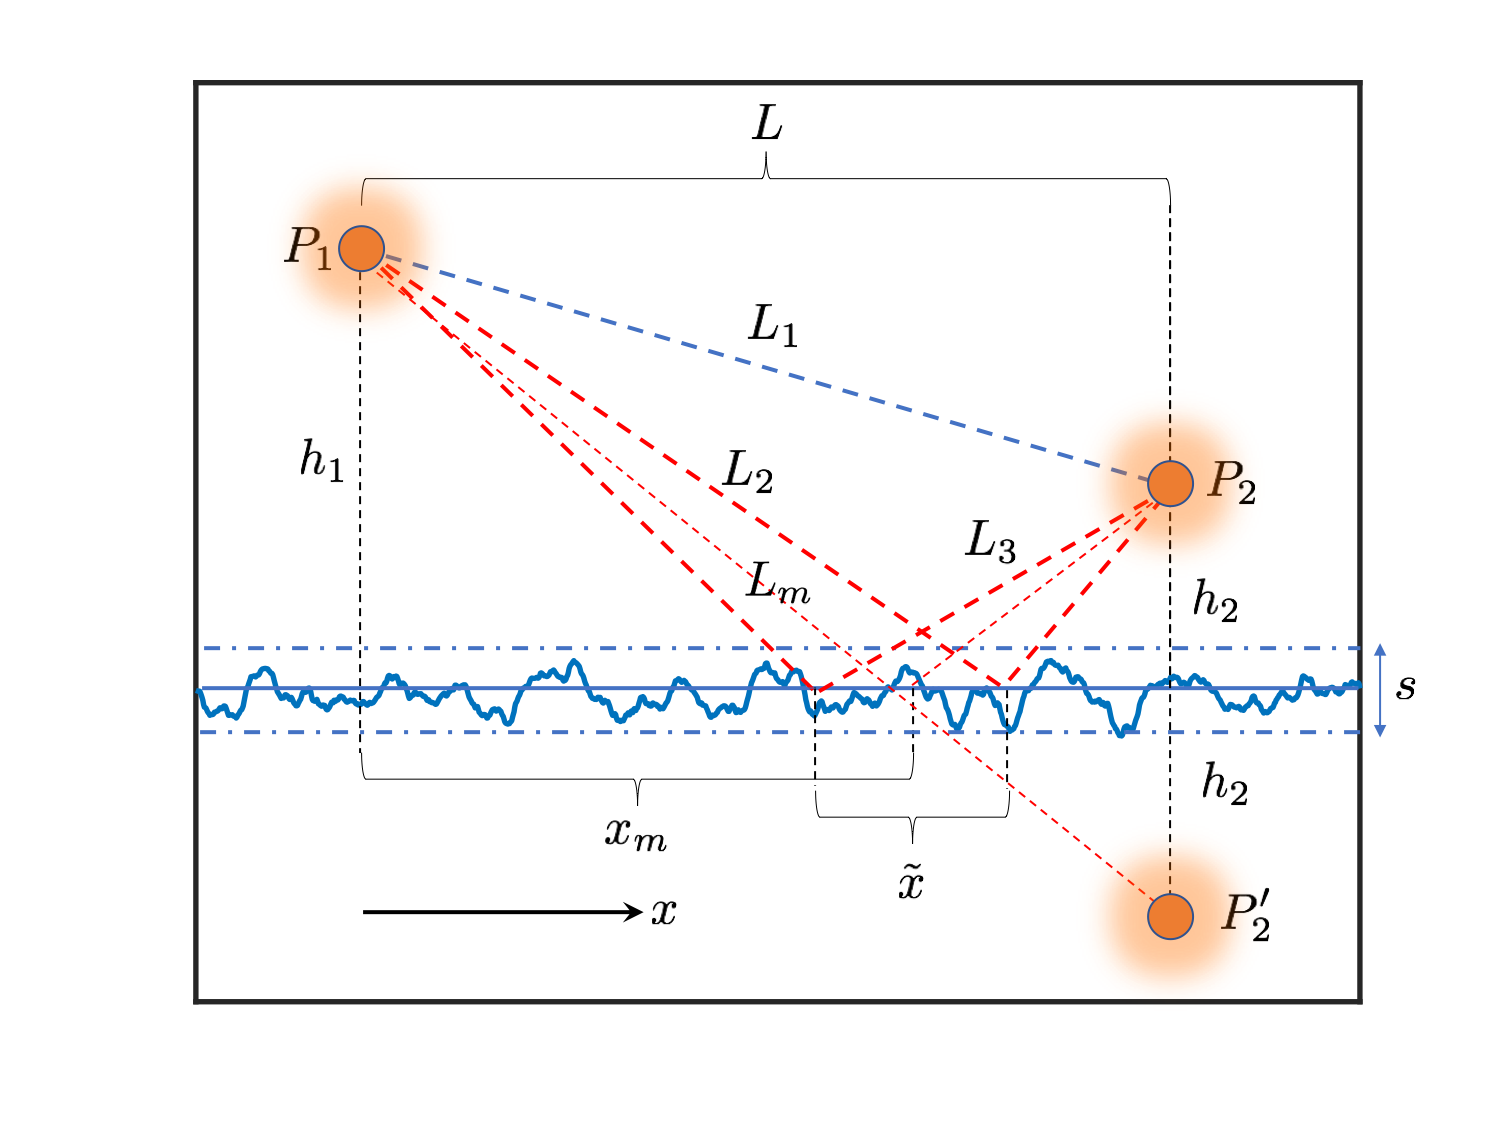
\includegraphics[width=5in]{../media/analysis/multipath_layout.png}
  
  \renewcommand{\baselinestretch}{1} \small\normalsize
  \begin{quote}
    \caption[Geometry for Diffraction Along the Sea Surface]{Geometry for Diffraction Along the Sea Surface\label{gf_fig:15}}
  \end{quote}
\end{figure}
\renewcommand{\baselinestretch}{2} \small\normalsize

\noindent We can simplify the various path lengths through a binomial expansion. 

\begin{equation}
\begin{aligned}
L_1 & = \sqrt{L^2 + (h_1-h_2)^2}  \approx L + \frac{(h_1 - h_2)^2}{2L}\\
L_m & = \sqrt{L^2 + (h_1+h_2)^2}  \approx L + \frac{(h_1 + h_2)^2}{2L}\\
L_2 &= \sqrt{x^2 + \left( h_1 - s(x)\right)^2}  \approx x + \frac{(h_1-s(x))^2}{2x}\\
L_3 & = \sqrt{\left(L - x\right)^2 + \left( h_2 - s(x)\right)^2}  \approx L-x + \frac{(h_2 - s(x))^2}{2\left(L-x\right)}\\
\end{aligned}
\label{gf_eq:59}
\end{equation}
\renewcommand{\baselinestretch}{2} \small\normalsize

We can use Equation \ref{gf_eq:52} with the paraxial Green's function where the surface normal is now given as $\hat{z}$. The reflected wave along $L_3$ will then be given by

\begin{equation}
\begin{aligned}
U(P_2) &= 2jk_p\int\limits_{0}^{L}dx\Gamma U(s)\frac{z}{x}\sqrt{\frac{1}{8\pi jk_p x}}\exp\left[-jk_p\left(x +\frac{z^2}{2x} \right) \right]\exp\left[-\frac{jk_pm}{2}x\right] \\
&= \int\limits_{0}^{L}dx\Gamma U(s)\frac{z}{x}\sqrt{\frac{jk_p}{2\pi x}}\exp\left[-jk_p\left(x +\frac{z^2}{2x} \right) \right]\exp\left[-\frac{jk_pm}{2}x\right] \\
\end{aligned}
\label{gf_eq:55}
\end{equation}
\renewcommand{\baselinestretch}{2} \small\normalsize

From the geometry in Figure \ref{gf_fig:15}, we are shifting the starting point for the return path by $x$ and we need to let $x \rightarrow L-x$ and $z \rightarrow h_2-s$. We can also assume that $h_2 >> s$ and neglect the $s$ term in the amplitude so that we now have

\begin{equation}
\begin{aligned}
U_2(P_2) &= \int\limits_{0}^{L}dx\Gamma U(s)\frac{h_2}{L-x}\sqrt{\frac{jk_p}{2\pi (L-x)}}\exp\left[-jk_p\left(L-x +\frac{(h_2-s)^2}{2(L-x)} \right) \right]\exp\left[-\frac{jk_pm}{2}(L-x)\right] \\
&= \int\limits_{0}^{L}dx\Gamma U(s)\frac{h_2}{L-x}\sqrt{\frac{jk_p}{2\pi (L-x)}}\exp\left[-jk_pL_3\right]\exp\left[-\frac{jk_pm}{2}(L-x)\right] \\
\end{aligned}
\label{gf_eq:56}
\end{equation}
\renewcommand{\baselinestretch}{2} \small\normalsize

The reflected wave solution at the sea surface, $U_2(s)$, follows from the free space solution, where $z \rightarrow h_1-s$.

\begin{equation}
\begin{aligned}
U_2(s) &= \sqrt{\frac{1}{8\pi jk_px}}\exp\left[-jk_p\left(x+\frac{z^2}{2x} + \frac{m}{2}x\right)\right] \\
&=\sqrt{\frac{1}{8\pi jk_px}}\exp\left[-jk_pL_2\right]\exp\left[-\frac{jk_pm}{2}x\right] \\
\end{aligned}
\label{gf_eq:57}
\end{equation}
\renewcommand{\baselinestretch}{2} \small\normalsize

\noindent The full solution for the reflected wave is then 

\begin{equation}
\begin{aligned}
U_2(P_2) &= \int_0^L dx \Gamma \sqrt{\frac{1}{8\pi j k_p x}}\exp[-jk_pL_2]\frac{h_2}{L-x}\sqrt{\frac{jk_p}{2\pi(L-x)}}\exp[-jk_pL_3]\exp\left[-\frac{jk_pmL}{2}\right]\\
&= \frac{1}{4\pi}\exp\left[-\frac{jk_pmL}{2}\right]\int_0^L dx \Gamma \sqrt{\frac{1}{x}}\sqrt{\frac{1}{L-x}}\frac{h_2}{L-x}\exp\left[-jk_p\left(L_2+L_3\right) \right]
\label{gf_eq:58}
\end{aligned}
\end{equation}
\renewcommand{\baselinestretch}{2} \small\normalsize

In the paraxial approximation, the phase term with the index of refraction is dependent on the ground distance between the points, $L$, and not on $x$, so it can come out of the integral. This approach only captures the reflected portion of the field, to get the solution for the full field, we need to use superposition and add the solution for the direct path.

\begin{equation}
\begin{gathered}
U(P_2) = U_1(P_2) + U_2(P_2)\\
= \sqrt{\frac{1}{8\pi jk_pL}}\exp\left[-jk_pL_1\right]\exp\left[-\frac{jk_pmL}{2}\right] \\
+ \frac{1}{4\pi}\exp\left[-\frac{jk_pmL}{2}\right]\int_0^L dx \Gamma \sqrt{\frac{1}{x}}\sqrt{\frac{1}{L-x}}\frac{h_2}{L-x}\exp\left[-jk_p\left(L_2+L_3\right) \right]
\label{gf_eq:58a}
\end{gathered}
\end{equation}
\renewcommand{\baselinestretch}{2} \small\normalsize

\subsubsection{Asymptotic Approximation}
We can now look at an asymptotic approach to solve Equation \ref{gf_eq:58a}. The path length for a given reflected ray, $L_r$ is given by

\begin{equation}
\begin{aligned}
L_r &= L_2 + L_3 \\
& = x + \frac{h_1^2-2h_1s(x)}{2x} +  L-x + \frac{h_2^2 - 2h_2s(x)}{2\left(L-x\right)} \\
& = L + \frac{1}{2}\left[\frac{h_1^2}{x} + \frac{h_2^2}{L-x} \right] - s(x)\left[ \frac{h_1}{x} + \frac{h_2}{L-x}\right] \\
&= L + L_0 - L_s
\end{aligned}
\label{gf_eq:60}
\end{equation}
\renewcommand{\baselinestretch}{2} \small\normalsize

Here $L_0$ represents the deterministic component and $L_s$ represents the random component. The primary reflection point, $x_m$, should be a saddle point and provide the dominant contribution. We can therefore perform a Taylor expansion of $L_0$ about $x_m$.

\begin{equation}
\begin{gathered}
\label{gf_eq:61}
L_0 \approx L_0(x_m) + \frac{1}{2}\frac{d^2L_0}{dx^2}\bigg|_{x_m}(x-x_m)^2 \\
\frac{dL_0}{dx} = \frac{1}{2}\left[\frac{-h_1^2}{x^2} + \frac{h_2^2}{(L-x)^2} \right]\\
\frac{d^2L_0}{dx^2} = \frac{h_1^2}{x^3} + \frac{h_2^2}{(L-x)^3} 
\end{gathered}
\end{equation}
\renewcommand{\baselinestretch}{2} \small\normalsize

\noindent Since $\frac{dL_0}{dx}\big|_{x_m} = 0$, we can solve for $x_m$

\begin{equation}
\begin{gathered}
x_m = \frac{h_1L}{h_1+h_2}
\end{gathered}
\label{gf_eq:64}
\end{equation}
\renewcommand{\baselinestretch}{2} \small\normalsize

\noindent This gives the following Taylor series terms:

\begin{equation}
\begin{aligned}
L_0(x_m) &= \frac{(h_1+h_2)^2}{2L} \\
L_0''=\frac{d^2L_0}{dx^2}\bigg|_{x_m}  &= \frac{(h_1+h_2)^4}{h_1h_2L^3} \\
L_s(x_m) &= \frac{2s(x)(h_1 + h_2)}{L}\\
\end{aligned}
\label{gf_eq:65}
\end{equation}
\renewcommand{\baselinestretch}{2} \small\normalsize

\noindent The expansion of $L_0$ to second order is then

\begin{equation}
L_0 \approx \frac{(h_1+h_2)^2}{2L} + \frac{(h_1+h_2)^4}{2h_1h_2L^3}(x-x_m)^2
\label{gf_eq:66}
\end{equation}
\renewcommand{\baselinestretch}{2} \small\normalsize

\noindent We can now substitute this into the exponential term of the integral in Equation \ref{gf_eq:58}

\begin{equation}
\begin{aligned}
&\exp\left[-jk_p\left( L+L_0-L_s\right) \right]\\
&= \exp\left[-jk_p\left( L+L_0(x_m) + \frac{L_0''}{2}(x-x_m)^2-L_s\right) \right]\\
&= \exp\left[-jk_p\left( L+\frac{(h_1+h_2)^2}{2L} + \frac{L_0''}{2}(x-x_m)^2-L_s\right)\right]\\
&=\exp\left[-jk_p\left(L_m+\frac{L_0''}{2}(x-x_m)^2-L_s\right)\right]\\
\label{gf_eq:67}
\end{aligned}
\end{equation}
\renewcommand{\baselinestretch}{2} \small\normalsize

\noindent We can substitute in for $L_m$ and continue simplifying.

\begin{equation}
\begin{aligned}
&\exp\left[-jk_p\left(L_m+\frac{L_0''}{2}(x-x_m)^2-L_s\right)\right]\\
&=\exp\left[-jk_pL_m\right]\exp\left[-jk_p\left(\frac{L_0''}{2}(x-x_m)^2-L_s\right)\right]\\
&=\exp\left[-jk_pL_m\right]\exp\left[\frac{-jk_pL_0''}{2}(x-x_m)^2\right]\exp\left[jk_pL_s \right]\\
\label{gf_eq:67a}
\end{aligned}
\end{equation}
\renewcommand{\baselinestretch}{2} \small\normalsize

Because $L_m$ is not dependent on $x$, it can come outside of the integral. If we assume that $L_s$ is locally sinusoidal with amplitude $\sigma$, frequency $k_{\omega}$, and phase $\theta$, we can approximate the exponential term as 

\begin{equation}
\begin{aligned}
\exp\left[jk_pL_s\right] =\exp\left[j\sigma \sin\left(k_{\omega} (x-x_m) + \theta\right) \right]
\end{aligned}
\label{gf_eq:68}
\end{equation}
\renewcommand{\baselinestretch}{2} \small\normalsize

\noindent From Equation \ref{gf_eq:65}, the random amplitude, $\sigma$, is given by

\begin{equation}
\begin{aligned}
\sigma = k_pL_s = \frac{2k_ps(h_1+h_2)}{L}
\end{aligned}
\label{gf_eq:69}
\end{equation}
\renewcommand{\baselinestretch}{2} \small\normalsize

We can then use the Jacobi-Anger expansion \cite{gbur_math} to convert the exponential term into an infinite sum of Bessel functions.

\begin{equation}
\begin{aligned}
& \exp\left[j\sigma \sin\left(k_{\omega} (x-x_m) + \theta\right) \right] \\ &=\sum_{l=-\infty}^{\infty}J_l(\sigma)\exp\left[jl(k_{\omega}(x-x_m) + \theta) \right] \\
&=\sum_{l=-\infty}^{\infty}J_l(\sigma)\exp\left[jl\theta\right]\exp\left[jlk_{\omega}(x-x_m)\right] 
\end{aligned}
\label{gf_eq:70}
\end{equation}
\renewcommand{\baselinestretch}{2} \small\normalsize

\noindent We can now rewrite Equation \ref{gf_eq:67} as

\begin{equation}
\begin{gathered}
\exp\left[-jk_p\left( L_2 + L_3\right) \right]= \\
\exp\left[-jk_pL_m\right]\sum_{l=-\infty}^{\infty}J_l(\sigma)\exp\left[jl\theta\right]
\exp\left[-\frac{jk_pL_0''}{2}(x-x_m)^2+jlk_{\omega}(x-x_m)\right]\\
\label{gf_eq:98}
\end{gathered}
\end{equation}
\renewcommand{\baselinestretch}{2} \small\normalsize

Only the last exponential term is dependent on $x$, so the other terms will come out of the integral. We can let $\tilde{x} = x-x_m$ for clarity and then simplify the last exponential by completing the square.

\begin{equation}
\begin{aligned}
&\frac{-jk_pL_0''}{2}\tilde{x}^2+jlk_{\omega}\tilde{x}\\
&=-\frac{jk_pL_0''}{2}\left[\tilde{x}^2 - \frac{2lk_{\omega}}{k_pL_0''}\tilde{x} \right]\\
&=-\frac{jk_pL_0''}{2}\left[\left(x-\frac{lk_{\omega}}{k_pL_0''} \right)^2 + \frac{l^2k_{\omega}^2}{k_p^2L_0''^2} \right]\\
&=-\frac{jk_pL_0''}{2}\left(x-\frac{lk_{\omega}}{k_pL_0''} \right)^2 - \frac{jl^2k_{\omega}^2}{k_pL_0''} 
\label{gf_eq:99}
\end{aligned}
\end{equation}
\renewcommand{\baselinestretch}{2} \small\normalsize

\noindent Equation \ref{gf_eq:98} can now be rewritten as

\begin{equation}
\begin{gathered}
\exp\left[-jk_p\left( L_2 + L_3\right) \right]= \\
\exp\left[-jk_pL_m\right]\sum_{l=-\infty}^{\infty}J_l(\sigma)\exp\left[jl\theta\right]
\exp\left[- \frac{jl^2k_{\omega}^2}{k_pL_0''} \right]\exp\left[-\frac{jk_pL_0''}{2}\left(\tilde{x}-\frac{lk_{\omega}}{2k_pL_0''} \right)^2\right]\\
\label{gf_eq:100}
\end{gathered}
\end{equation}
\renewcommand{\baselinestretch}{2} \small\normalsize

\noindent We can make a further substitution and introduce the variable $\phi_l$

\begin{equation}
\phi_l = l\theta - \frac{l^2k_{\omega}^2}{2k_pL_0''}
\label{gf_eq:101}
\end{equation}
\renewcommand{\baselinestretch}{2} \small\normalsize

\noindent We are now in position to rewrite Equation \ref{gf_eq:58} as

\begin{equation}
\begin{gathered}
U_2(P_2) = \frac{1}{4\pi} \exp[-jk_pL_m] \exp\left[-\frac{jk_pmL}{2}\right]\sum_{l=-\infty}^{\infty}J_l(\sigma)\exp\left[j\phi_l\right] \\
\times \int_0^L  \Gamma \sqrt{\frac{1}{x}}\sqrt{\frac{1}{L-x}}\frac{h_2}{L-x}\exp\left[-\frac{jk_pL_0''}{2}\left([x-x_m]-\frac{lk_{\omega}}{k_pL_0''} \right)^2\right]
\label{gf_eq:102}
\end{gathered}
\end{equation}
\renewcommand{\baselinestretch}{2} \small\normalsize

As we have seen previously, the quadratic phase term rapidly oscillates as $x$ moves away from $x_m$, so we can let the integration limits go to $\pm \infty$ and find an asymptotic solution \cite{cheng_analytic_methods}. The amplitudes will be replaced by their values at $x_m$, which results in the following expression.

\begin{equation}
\begin{gathered}
U_2(P_2) = \frac{1}{4\pi} \exp[-jk_pL_m] \exp\left[-\frac{jk_pmL}{2}\right] \sum_{l=-\infty}^{\infty}J_l(\sigma)\exp\left[j\phi_l\right]\  \\
\times \Gamma_1 \sqrt{\frac{1}{x_m}}\sqrt{\frac{1}{L-x_m}}\frac{h_2}{L-x_m}\sqrt{\frac{\pi 2}{jk_pL_0''}}
\label{gf_eq:72}
\end{gathered}
\end{equation}
\renewcommand{\baselinestretch}{2} \small\normalsize

\noindent Substituting in for $x_m$ and $L_0''$ yields the final asymptotic result for the reflected wave.

\begin{equation}
U_2(P_2) = \sqrt{\frac{1}{8\pi jk_p L}}\Gamma_1e^{-jk_pL_m} e^{-\frac{jk_pmL}{2}} \sum_{l=-\infty}^{\infty}J_l(\sigma)e^{j\phi_l}
\label{gf_eq:73}
\end{equation}
\renewcommand{\baselinestretch}{2} \small\normalsize

A simple plane wave solution would result in $U_2(P_2) = \Gamma_1\exp[-jk_pL_m]$ for the reflected wave. Here, we see that the deterministic component from the paraxial wave  solution scales the plane wave solution by the geometric spreading of a paraxial wave. The random sea height contributions are now contained in the sum of Bessel functions. We can now add the solution for the direct wave for the asymptotic solution for the full field.

\begin{equation}
\boxed{U(P_2) = \sqrt{\frac{1}{8\pi jk_p L}}e^{-\frac{jk_pmL}{2}} \left[e^{-jk_pL_1}+\Gamma_1e^{-jk_pL_m} \sum_{l=-\infty}^{\infty}J_l(\sigma)e^{j\phi_l}\right]}
\label{gf_eq:73a}
\end{equation}
\renewcommand{\baselinestretch}{2} \small\normalsize

Equation \ref{gf_eq:73a} is a significant result as the asymptotic expression allows us to look at the impact of random wave heights on the average field at the observation point, although it is really only valid only under a flat earth approximation. We can however, implement this in a numerical method similar to ray tracing that allows $m$ to vary as a function of $z$.

It is often convenient to work with a propagation factor, $F_p$ instead of the field. The propagation factor acts as a multiplier on the direct path and is really just Equation \ref{gf_eq:73a} normalized by the amplitude for the direct path. For the paraxial wave assumption, the propagation factor is the same as what we would have gotten from using plane waves.

\begin{equation}
F_p = e^{-jk_pL_1}+\Gamma_1e^{-jk_pL_m} \sum_{l=-\infty}^{\infty}J_l(\sigma)e^{j\phi_l}
\label{gf_eq:73ab}
\end{equation}
\renewcommand{\baselinestretch}{2} \small\normalsize

\subsection{Cylindrical Waves}\label{cylindrical_diffraction}
The analysis here will rely extensively on the work presented in Section \ref{paraxial_diffraction}, but we will use cylindrical waves instead of paraxial waves. We will again use the geometry shown in Figure \ref{gf_fig:15}, and will work with the 2-D free space Green's function.

\begin{equation}
G\left(\boldsymbol{\rho},\boldsymbol{\rho}'\right) = -\frac{j}{4}H_0^{(2)}\left(k_o|\boldsymbol{\rho} - \boldsymbol{\rho}' | \right)
\label{cyl_eq:1}
\end{equation}
\renewcommand{\baselinestretch}{2} \small\normalsize

\subsubsection{Integral Solution for Reflected Ray}
We can again use Equation \ref{gf_eq:52} with the Green's function given in Equation \ref{cyl_eq:1}. The surface normal is still given as $\hat{z}$, so we will only need to take the derivative with respect to $\rho$.
 
\begin{equation}
\begin{aligned}
U_2(P_2) &= -2\oint_s ds U_2(s)\hat{n}\cdot\nabla G\\
&= -2\int_0^L dx \Gamma U_2(s)\cos(\phi)\frac{\partial G}{\partial \rho}\\
\end{aligned}
\label{cyl_eq:6}
\end{equation}
\renewcommand{\baselinestretch}{2} \small\normalsize

We can use the fact that $\partial H_0^{(2)}(k_o\rho)/\partial \rho = -k_oH_1^{(2)}(k_o\rho)$ and let $\rho \rightarrow L_3$ and $\cos(\phi) \rightarrow h2/L_3$ to solve for $U_2(P_2)$.

\begin{equation}
\begin{aligned}
U_2(P_2) = -\frac{2j}{4}\int_0^L dx \Gamma U_2(s)k_o\frac{h_2}{L_3}H_1^{(2)}(k_oL_3)\\
\label{cyl_eq:7}
\end{aligned}
\end{equation}
\renewcommand{\baselinestretch}{2} \small\normalsize

\noindent We can now substitue the asymptotic expression for $H_1^{(2)}$

\begin{equation}
\begin{aligned}
U_2(P_2) &= -\frac{jk_o}{2}\int_0^L dx \Gamma U_2(s)\frac{h_2}{L_3}\sqrt{\frac{2}{\pi k_o L_3}}e^{-j(k_oL_3-3\pi /4)}\\
&= -\frac{jk_o}{2}\sqrt{\frac{2}{\pi k_o}}\int_0^L dx \Gamma U_2(s)\frac{h_2}{L_3}\frac{1}{\sqrt{L_3}}e^{-j(k_oL_3-3\pi /4)} \\
\label{cyl_eq:7b}
\end{aligned}
\end{equation}
\renewcommand{\baselinestretch}{2} \small\normalsize

\noindent We can factor out the  $e^{j3\pi /4} = j\sqrt{j}$ term.

\begin{equation}
\begin{aligned}
U_2(P_2) &= -j\sqrt{\frac{k_o}{2\pi}}e^{j3\pi /4}\int_0^L dx \Gamma U_2(s)\frac{h_2}{L_3}\frac{1}{\sqrt{L_3}}e^{-jk_oL_3} \\
&= \sqrt{\frac{j k_o}{2\pi}}\int_0^L dx \Gamma U_2(s)\frac{h_2}{L_3}\frac{1}{\sqrt{L_3}}e^{-jk_oL_3} \\
\label{cyl_eq:7ba}
\end{aligned}
\end{equation}
\renewcommand{\baselinestretch}{2} \small\normalsize

\noindent The solution at the sea surface, $U_2(s)$ follows again from the free space solution. Here we will let $\rho \rightarrow L_2$ and substitute the asymptotic expression for $H_0^{(2)}$.

 \begin{equation}
\begin{aligned}
U_2(s) &= -\frac{j}{4}H_0^{(2)}(k_o L_2) \\
&= -\frac{j}{4}\sqrt{\frac{2}{\pi k_o L_2}}e^{-jk_oL_2 -\pi/4}\\
\label{cyl_eq:7c}
\end{aligned}
\end{equation}
\renewcommand{\baselinestretch}{2} \small\normalsize

\noindent We can again factor out the $e^{j\pi/4} = \sqrt{j}$ term.
 \begin{equation}
\begin{aligned}
U_2(s) &= -j\sqrt{\frac{1}{8\pi k_oj L_2}}e^{j\pi/4}e^{-jk_oL_2} \\
&= \sqrt{\frac{1}{8 \pi k_o j L_2}}e^{-jk_oL_2} \\
\label{cyl_eq:7ca}
\end{aligned}
\end{equation}
\renewcommand{\baselinestretch}{2} \small\normalsize

\noindent The full solution for the reflected wave is then

\begin{equation}
\begin{aligned}
U_2(P_2) &= \sqrt{\frac{j k_o}{2\pi}}\int_0^L dx \Gamma \sqrt{\frac{1}{8 \pi k_o j L_2}}e^{-jk_oL_2}  \frac{h_2}{L_3}\frac{1}{\sqrt{L_3}}e^{-jk_oL_3} \\
&= \frac{1}{4\pi} \int_0^L dx \Gamma \frac{1}{\sqrt{L_2L_3}}\frac{h_2}{L_3} e^{-jk_o(L_2+L_3)}
\label{cyl_eq:7d}
\end{aligned}
\end{equation}
\renewcommand{\baselinestretch}{2} \small\normalsize

Equation \ref{cyl_eq:7d} is very similar to Equation \ref{gf_eq:58}. The differences are now that the denominators have the actual path lengths instead of just the distance along the $x$ axis.

\subsubsection{Asymptotic Approximation}
Because the exponential term in the integral is the same, we will use the same asymptotic approximations used in Section \ref{paraxial_diffraction}. With these assumptions applied, we can rewrite Equation \ref{cyl_eq:7d} as

\begin{equation}
\begin{gathered}
U_2(P_2) = \frac{1}{4\pi} \exp[-jk_oL_m] \sum_{l=-\infty}^{\infty}J_l(\sigma)\exp\left[j\phi_l\right] \\
\times \int_0^L  \Gamma \frac{1}{\sqrt{L_2L_3}}\frac{h_2}{L_3}\exp\left[-\frac{jk_oL_0''}{2}\left([x-x_m]-\frac{lk_{\omega}}{k_oL_0''} \right)^2\right]
\label{cyl_eq:8}
\end{gathered}
\end{equation}
\renewcommand{\baselinestretch}{2} \small\normalsize

\noindent The asymptotic solution is then

\begin{equation}
\begin{gathered}
U_2(P_2) = \frac{1}{4\pi} \exp[-jk_oL_m] \sum_{l=-\infty}^{\infty}J_l(\sigma)\exp\left[j\phi_l\right]\  \\
\times \Gamma_1 \frac{1}{\sqrt{L_2(x_m)L_3(x_m)}}\frac{h_2}{L_3(x_m)}\sqrt{\frac{\pi 2}{jk_oL_0''}}
\label{cyl_eq:9}
\end{gathered}
\end{equation}
\renewcommand{\baselinestretch}{2} \small\normalsize

\noindent Expanding $L_0''$ and collecting terms yields

\begin{equation}
\begin{gathered}
U_2(P_2) = \sqrt{\frac{1}{8\pi j k_o}} \exp[-jk_oL_m] \sum_{l=-\infty}^{\infty}J_l(\sigma)\exp\left[j\phi_l\right]\  \\
\times \Gamma_1 \frac{1}{\sqrt{L_2(x_m)L_3(x_m)}}\frac{h_2\sqrt{h_1h_2L^3}}{L_3(x_m)(h_1+h_2)^2}
\label{cyl_eq:10}
\end{gathered}
\end{equation}
\renewcommand{\baselinestretch}{2} \small\normalsize

\noindent Substituting in for $x_m$ and performing some extensive algebraic manipulation yields the final asymptotic solution

\begin{equation}
U_2(P_2) = \sqrt{\frac{1}{8\pi j k_oL_m}} \Gamma_1\exp[-jk_oL_m] \sum_{l=-\infty}^{\infty}J_l(\sigma)\exp\left[j\phi_l\right]
\label{cyl_eq:11}
\end{equation}
\renewcommand{\baselinestretch}{2} \small\normalsize

Adding in the direct path solution gives us the full field description.

\begin{equation}
\boxed{U(P_2) = \sqrt{\frac{1}{8\pi j k_o}}\left[\frac{1}{\sqrt{L_1}} e^{-jk_oL_1}+\Gamma_1\frac{1}{\sqrt{L_m}} e^{-jk_oL_m} \sum_{l=-\infty}^{\infty}J_l(\sigma)e^{j\phi_l}\right]}
\label{cyl_eq:12}
\end{equation}
\renewcommand{\baselinestretch}{2} \small\normalsize

Equation \ref{cyl_eq:12} is again very similar to Equation \ref{gf_eq:73a}, where we now have the cylindrical spreading for each wave based on the path lengths. We can again normalize this equation by the direct path amplitude to get the propagation factor.

\begin{equation}
F_p =e^{-jk_oL_1}+\Gamma_1\sqrt{\frac{L_1}{L_m}} e^{-jk_oL_m} \sum_{l=-\infty}^{\infty}J_l(\sigma)e^{j\phi_l}
\label{cyl_eq:13}
\end{equation}
\renewcommand{\baselinestretch}{2} \small\normalsize

\subsection {Knife Edges and Non-planar Terrain}
In many cases of interest, the surface we want to propagate over is not planar. In this case, we cannot use the Rayleigh-Sommerfeld approach with the earth as the surface. However, we can formulate the diffraction integral in altitude (perpendicular to the surface) and treat subsequent obstacles as knife edges \cite{whitteker_diffraction}. If we treat the knife edge as an aperture that starts at $z=\xi$, assume no $y$ dependence from the source, $U(x,y) = U(x)$, and let propagation be along the $x$ axis, we can integrate out the $y$ dependence from the Fresnel diffraction equation (Equation \ref{gf_eq:53d}) and rewrite it as 

\begin{equation}
\begin{aligned}
U(P_2) &=\frac{je^{-jk_ox}}{\lambda x}\int_{\xi}^{\infty}\int_{-\infty}^{\infty} U(z') \exp\left[-j \frac{k_o}{2x}\left(z-z'\right)^2 \right]   \exp\left[-j \frac{k_o}{2x}\left(y-y'\right)^2 \right]dz' dy' \\
&=\frac{je^{-jk_ox}}{\lambda x}\sqrt{\frac{\pi 2 x}{jk_o}}\int_{\xi}^{\infty}U(z') \exp\left[-j \frac{k_o}{2x}\left(z-z'\right)^2 \right]dz'\\
\end{aligned}
\label{gf_eq:82}
\end{equation}
\renewcommand{\baselinestretch}{2} \small\normalsize

\noindent Substituting $\lambda = 2\pi/k_o$ yields the final result.

\begin{equation}
\begin{aligned}
\boxed{U(P_2) =\sqrt{\frac{jk_o}{2\pi x}}e^{-jk_ox}\int_{\xi}^{\infty}U(z') \exp\left[-j \frac{k_o}{2x}\left(z-z'\right)^2 \right]dz'}\\
\end{aligned}
\label{gf_eq:82a}
\end{equation}
\renewcommand{\baselinestretch}{2} \small\normalsize

Because we are integrating in altitude, we have the full field solution and do not need to add in a direct path. Equation \ref{gf_eq:82a} can be used in a marching algorithm that steps along the $x$ axis, solving in $z$.

\section{Diffraction from a Curved Earth}
This section discusses the use of Green's functions to describe propagating over the earth where the earth is allowed to be curved.

\subsection{Fourier Split Step Marching Method for PWE}
The typical PWE solution is formulated as a marching algorithm and will be derived here using the Green's function method and directly from the differential equation. 

\subsubsection{Derivation from Green's Function}
As we saw in the development of the PWE, the dependence on the index of refraction can be factored out into a separate phase term. We can replace $k_o$ in Equation \ref{gf_eq:82a} with $k_p$ and then multiply it by the additional phase. We can also extend the lower limit of the integral to $-\infty$ for generality.

\begin{equation}
U(P_2) =\sqrt{\frac{jk_p}{2\pi x}}e^{-jk_px\left(1+\frac{m}{2}\right)}\int_{\xi}^{\infty}U(z') \exp\left[-j \frac{k_p}{2x}\left(z-z'\right)^2 \right]dz'
\label{gf_eq:301}
\end{equation}
\renewcommand{\baselinestretch}{2} \small\normalsize

Because this is a convolution integral, and we can represent convolution in space as multiplication in Frequency, we can rewrite this as

\begin{equation}
\begin{aligned}
U(P_2) &=\sqrt{\frac{jk_p}{2\pi x}}e^{-jk_px\left(1+\frac{m}{2}\right)}\mathcal{F}^{-1}\left\{\mathcal{F}\{U(z')\}\mathcal{F}\left\{ \exp\left[-j \frac{k_p}{2x}\left(z-z'\right)^2 \right]\right\} \right\} \\
&=\sqrt{\frac{jk_p}{2\pi x}}e^{-jk_px\left(1+\frac{m}{2}\right)}\mathcal{F}^{-1}\left\{\mathcal{F}\{U(z')\}\sqrt{\frac{2\pi x}{jk_p}}\exp\left[-j\frac{k_z^2}{2k_p}x \right] \right\} \\
\label{gf_eq:302}
\end{aligned}
\end{equation}
\renewcommand{\baselinestretch}{2} \small\normalsize

\noindent Combining terms and simplifying gives the final result

\begin{equation}
\begin{aligned}
U(P_2) = e^{-jk_px\left(1+\frac{m}{2}\right)}\mathcal{F}^{-1}\left\{\mathcal{F}\{U(z')\}\exp\left[-j\frac{k_z^2}{2k_p}x \right] \right\} \\
\label{gf_eq:303}
\end{aligned}
\end{equation}
\renewcommand{\baselinestretch}{2} \small\normalsize


\subsubsection{Derivation from PWE}
\noindent The most straight forward approach is to start by taking the Fourier transform of the PWE (Equation \ref{gf_eq:76}) along $z$

\begin{equation}
-k_z^2\hat{A} -2jk_p\frac{\partial \hat{A}}{\partial x} +k_p^2m\hat{A}
\label{gf_eq:77}
\end{equation}
\renewcommand{\baselinestretch}{2} \small\normalsize

\noindent This has the solution

\begin{equation}
\begin{aligned}
\hat{A}(x,k_z) &= \hat{A}(0,k_z)\exp\left[-j\frac{k_p^2m-k_z^2}{2k_p}x \right] \\
&= \hat{A}(0,k_z)\exp\left[-j\frac{k_pm}{2}x\right]\exp\left[j\frac{k_z^2}{2k_p}x \right]
\end{aligned}
\label{gf_eq:78}
\end{equation}
\renewcommand{\baselinestretch}{2} \small\normalsize

We will next take the inverse Fourier transform along $z$ of Equation \ref{gf_eq:78}, which we can write as

\begin{equation}
\begin{aligned}
A(x,z) &= \mathcal{F}^{-1}\left\{\hat{A}(x,k_z) \right\} \\
&= \exp\left[-j\frac{k_pm}{2}x\right]\mathcal{F}^{-1}\left\{\exp\left[j\frac{k_z^2}{2k_p}x \right]\hat{A}(0,k_z) \right\}
\end{aligned}
\label{gf_eq:79}
\end{equation}
\renewcommand{\baselinestretch}{2} \small\normalsize

\noindent We can convert Equation \ref{gf_eq:79} into a marching algorithm by letting $x\rightarrow \Delta x = x-x_o$.

\begin{equation}
\boxed{A(x,z) = \exp\left[-j\frac{k_pm}{2}\Delta x\right]\mathcal{F}^{-1}\left\{\exp\left[j\frac{k_z^2}{2k_p}\Delta x \right]\hat{A}(x_o,k_z) \right\}}
\label{gf_eq:80}
\end{equation}
\renewcommand{\baselinestretch}{2} \small\normalsize

Equation \ref{gf_eq:80} is the split step algorithm that solves for the modulation amplitude in the PWE. As shown previously, to get the full field we would need to multiply by $e^-jk_px$.